%%
%% Automatically generated file from DocOnce source
%% (https://github.com/hplgit/doconce/)
%%
%%


%-------------------- begin preamble ----------------------

\documentclass[%
oneside,                 % oneside: electronic viewing, twoside: printing
final,                   % draft: marks overfull hboxes, figures with paths
10pt]{article}

\listfiles               %  print all files needed to compile this document

\usepackage{relsize,makeidx,color,setspace,amsmath,amsfonts,amssymb}
\usepackage[table]{xcolor}
\usepackage{bm,ltablex,microtype}

\usepackage[pdftex]{graphicx}

\usepackage{fancyvrb} % packages needed for verbatim environments
\usepackage{minted}
\usemintedstyle{default}

\usepackage[T1]{fontenc}
%\usepackage[latin1]{inputenc}
\usepackage{ucs}
\usepackage[utf8x]{inputenc}

\usepackage{lmodern}         % Latin Modern fonts derived from Computer Modern

% Hyperlinks in PDF:
\definecolor{linkcolor}{rgb}{0,0,0.4}
\usepackage{hyperref}
\hypersetup{
    breaklinks=true,
    colorlinks=true,
    linkcolor=linkcolor,
    urlcolor=linkcolor,
    citecolor=black,
    filecolor=black,
    %filecolor=blue,
    pdfmenubar=true,
    pdftoolbar=true,
    bookmarksdepth=3   % Uncomment (and tweak) for PDF bookmarks with more levels than the TOC
    }
%\hyperbaseurl{}   % hyperlinks are relative to this root

\setcounter{tocdepth}{2}  % levels in table of contents

% Tricks for having figures close to where they are defined:
% 1. define less restrictive rules for where to put figures
\setcounter{topnumber}{2}
\setcounter{bottomnumber}{2}
\setcounter{totalnumber}{4}
\renewcommand{\topfraction}{0.95}
\renewcommand{\bottomfraction}{0.95}
\renewcommand{\textfraction}{0}
\renewcommand{\floatpagefraction}{0.75}
% floatpagefraction must always be less than topfraction!
% 2. ensure all figures are flushed before next section
\usepackage[section]{placeins}
% 3. enable begin{figure}[H] (often leads to ugly pagebreaks)
%\usepackage{float}\restylefloat{figure}

% --- fancyhdr package for fancy headers ---
\usepackage{fancyhdr}
\fancyhf{} % sets both header and footer to nothing
\renewcommand{\headrulewidth}{0pt}
\fancyfoot[LE,RO]{\thepage}
% Ensure copyright on titlepage (article style) and chapter pages (book style)
\fancypagestyle{plain}{
  \fancyhf{}
  \fancyfoot[C]{{\footnotesize \copyright\ 1999-2018, Morten Hjorth-Jensen. Released under CC Attribution-NonCommercial 4.0 license}}
%  \renewcommand{\footrulewidth}{0mm}
  \renewcommand{\headrulewidth}{0mm}
}
% Ensure copyright on titlepages with \thispagestyle{empty}
\fancypagestyle{empty}{
  \fancyhf{}
  \fancyfoot[C]{{\footnotesize \copyright\ 1999-2018, Morten Hjorth-Jensen. Released under CC Attribution-NonCommercial 4.0 license}}
  \renewcommand{\footrulewidth}{0mm}
  \renewcommand{\headrulewidth}{0mm}
}

\pagestyle{fancy}


\usepackage[framemethod=TikZ]{mdframed}

% --- begin definitions of admonition environments ---

% --- end of definitions of admonition environments ---

% prevent orhpans and widows
\clubpenalty = 10000
\widowpenalty = 10000

% --- end of standard preamble for documents ---


% insert custom LaTeX commands...

\raggedbottom
\makeindex
\usepackage[totoc]{idxlayout}   % for index in the toc
\usepackage[nottoc]{tocbibind}  % for references/bibliography in the toc

%-------------------- end preamble ----------------------

\begin{document}

% matching end for #ifdef PREAMBLE

\newcommand{\exercisesection}[1]{\subsection*{#1}}


% ------------------- main content ----------------------



% ----------------- title -------------------------

\thispagestyle{empty}

\begin{center}
{\LARGE\bf
\begin{spacing}{1.25}
Data Analysis and Machine Learning: Neural networks, from the simple perceptron to deep learning and convolutional networks
\end{spacing}
}
\end{center}

% ----------------- author(s) -------------------------

\begin{center}
{\bf Morten Hjorth-Jensen${}^{1, 2}$} \\ [0mm]
\end{center}

\begin{center}
% List of all institutions:
\centerline{{\small ${}^1$Department of Physics, University of Oslo}}
\centerline{{\small ${}^2$Department of Physics and Astronomy and National Superconducting Cyclotron Laboratory, Michigan State University}}
\end{center}
    
% ----------------- end author(s) -------------------------

% --- begin date ---
\begin{center}
Oct 19, 2018
\end{center}
% --- end date ---

\vspace{1cm}


% !split
\subsection*{Neural networks}

Artificial neural networks are computational systems that can learn to
perform tasks by considering examples, generally without being
programmed with any task-specific rules. It is supposed to mimic a
biological system, wherein neurons interact by sending signals in the
form of mathematical functions between layers. All layers can contain
an arbitrary number of neurons, and each connection is represented by
a weight variable.


% !split
\subsection*{Artificial neurons}

The field of artificial neural networks has a long history of
development, and is closely connected with the advancement of computer
science and computers in general. A model of artificial neurons was
first developed by McCulloch and Pitts in 1943 to study signal
processing in the brain and has later been refined by others. The
general idea is to mimic neural networks in the human brain, which is
composed of billions of neurons that communicate with each other by
sending electrical signals.  Each neuron accumulates its incoming
signals, which must exceed an activation threshold to yield an
output. If the threshold is not overcome, the neuron remains inactive,
i.e.~has zero output.

This behaviour has inspired a simple mathematical model for an artificial neuron.

\begin{equation}
 y = f\left(\sum_{i=1}^n w_ix_i\right) = f(u)
 \label{artificialNeuron}
\end{equation}
Here, the output $y$ of the neuron is the value of its activation function, which have as input
a weighted sum of signals $x_i, \dots ,x_n$ received by $n$ other neurons.

Conceptually, it is helpful to divide neural networks into four
categories:
\begin{enumerate}
\item general purpose neural networks for supervised learning,

\item neural networks designed specifically for image processing, the most prominent example of this class being Convolutional Neural Networks (CNNs),

\item neural networks for sequential data such as Recurrent Neural Networks (RNNs), and

\item neural networks for unsupervised learning such as Deep Boltzmann Machines.
\end{enumerate}

\noindent
In natural science, DNNs and CNNs have already found numerous
applications. In statistical physics, they have been applied to detect
phase transitions in 2D Ising and Potts models, lattice gauge
theories, and different phases of polymers, or solving the
Navier-Stokes equation in weather forecasting.  Deep learning has also
found interesting applications in quantum physics. Various quantum
phase transitions can be detected and studied using DNNs and CNNs,
topological phases, and even non-equilibrium many-body
localization. Representing quantum states as DNNs quantum state
tomography are among some of the impressive achievements to reveal the
potential of DNNs to facilitate the study of quantum systems.

In quantum information theory, it has been shown that one can perform
gate decompositions with the help of neural. 

The applications are not limited to the natural sciences. There is a
plethora of applications in essentially all disciplines, from the
humanities to life science and medicine.

% !split
\subsection*{Neural network types}

An artificial neural network (ANN), is a computational model that
consists of layers of connected neurons, or nodes or units.  We will
refer to these interchangeably as units or nodes, and sometimes as
neurons.

It is supposed to mimic a biological nervous system by letting each
neuron interact with other neurons by sending signals in the form of
mathematical functions between layers.  A wide variety of different
ANNs have been developed, but most of them consist of an input layer,
an output layer and eventual layers in-between, called \emph{hidden
layers}. All layers can contain an arbitrary number of nodes, and each
connection between two nodes is associated with a weight variable.

Neural networks (also called neural nets) are neural-inspired
nonlinear models for supervised learning.  As we will see, neural nets
can be viewed as natural, more powerful extensions of supervised
learning methods such as linear and logistic regression and soft-max
methods we discussed earlier.


% !split
\subsection*{Feed-forward neural networks}

The feed-forward neural network (FFNN) was the first and simplest type
of ANNs that were devised. In this network, the information moves in
only one direction: forward through the layers.

Nodes are represented by circles, while the arrows display the
connections between the nodes, including the direction of information
flow. Additionally, each arrow corresponds to a weight variable
(figure to come).  We observe that each node in a layer is connected
to \emph{all} nodes in the subsequent layer, making this a so-called
\emph{fully-connected} FFNN.



% !split
\subsection*{Convolutional Neural Network}

A different variant of FFNNs are \emph{convolutional neural networks}
(CNNs), which have a connectivity pattern inspired by the animal
visual cortex. Individual neurons in the visual cortex only respond to
stimuli from small sub-regions of the visual field, called a receptive
field. This makes the neurons well-suited to exploit the strong
spatially local correlation present in natural images. The response of
each neuron can be approximated mathematically as a convolution
operation.  (figure to come)

Convolutional neural networks emulate the behaviour of neurons in the
visual cortex by enforcing a \emph{local} connectivity pattern between
nodes of adjacent layers: Each node in a convolutional layer is
connected only to a subset of the nodes in the previous layer, in
contrast to the fully-connected FFNN.  Often, CNNs consist of several
convolutional layers that learn local features of the input, with a
fully-connected layer at the end, which gathers all the local data and
produces the outputs. They have wide applications in image and video
recognition.

% !split
\subsection*{Recurrent neural networks}

So far we have only mentioned ANNs where information flows in one
direction: forward. \emph{Recurrent neural networks} on the other hand,
have connections between nodes that form directed \emph{cycles}. This
creates a form of internal memory which are able to capture
information on what has been calculated before; the output is
dependent on the previous computations. Recurrent NNs make use of
sequential information by performing the same task for every element
in a sequence, where each element depends on previous elements. An
example of such information is sentences, making recurrent NNs
especially well-suited for handwriting and speech recognition.

% !split
\subsection*{Other types of networks}

There are many other kinds of ANNs that have been developed. One type
that is specifically designed for interpolation in multidimensional
space is the radial basis function (RBF) network. RBFs are typically
made up of three layers: an input layer, a hidden layer with
non-linear radial symmetric activation functions and a linear output
layer (''linear'' here means that each node in the output layer has a
linear activation function). The layers are normally fully-connected
and there are no cycles, thus RBFs can be viewed as a type of
fully-connected FFNN. They are however usually treated as a separate
type of NN due the unusual activation functions.

% !split
\subsection*{Multilayer perceptrons}

One uses often so-called fully-connected feed-forward neural networks
with three or more layers (an input layer, one or more hidden layers
and an output layer) consisting of neurons that have non-linear
activation functions.

Such networks are often called \emph{multilayer perceptrons} (MLPs).

% !split
\subsection*{Why multilayer perceptrons?}

According to the \emph{Universal approximation theorem}, a feed-forward
neural network with just a single hidden layer containing a finite
number of neurons can approximate a continuous multidimensional
function to arbitrary accuracy, assuming the activation function for
the hidden layer is a \textbf{non-constant, bounded and
monotonically-increasing continuous function}.

Note that the requirements on the activation function only applies to
the hidden layer, the output nodes are always assumed to be linear, so
as to not restrict the range of output values.


% !split
\subsection*{Mathematical model}

The output $y$ is produced via the activation function $f$
\[
 y = f\left(\sum_{i=1}^n w_ix_i + b_i\right) = f(z),
\]
This function receives $x_i$ as inputs.
Here the activation $z=(\sum_{i=1}^n w_ix_i+b_i)$. 
In an FFNN of such neurons, the \emph{inputs} $x_i$ are the \emph{outputs} of
the neurons in the preceding layer. Furthermore, an MLP is
fully-connected, which means that each neuron receives a weighted sum
of the outputs of \emph{all} neurons in the previous layer.

% !split
\subsection*{Mathematical model}

First, for each node $i$ in the first hidden layer, we calculate a weighted sum $z_i^1$ of the input coordinates $x_j$,

\begin{equation} z_i^1 = \sum_{j=1}^{M} w_{ij}^1 x_j + b_i^1
\end{equation}

Here $b_i$ is the so-called bias which is normally needed in
case of zero activation weights or inputs. How to fix the biases and
the weights will be discussed below.  The value of $z_i^1$ is the
argument to the activation function $f_i$ of each node $i$, The
variable $M$ stands for all possible inputs to a given node $i$ in the
first layer.  We define  the output $y_i^1$ of all neurons in layer 1 as

\begin{equation}
 y_i^1 = f(z_i^1) = f\left(\sum_{j=1}^M w_{ij}^1 x_j  + b_i^1\right)
 \label{outputLayer1}
\end{equation}

where we assume that all nodes in the same layer have identical
activation functions, hence the notation $f$. In general, we could assume in the more general case that different layers have different activation functions.
In this case we would identify these functions with a superscript $l$ for the $l$-th layer,

\begin{equation}
 y_i^l = f^l(u_i^l) = f^l\left(\sum_{j=1}^{N_{l-1}} w_{ij}^l y_j^{l-1} + b_i^l\right)
 \label{generalLayer}
\end{equation}

where $N_l$ is the number of nodes in layer $l$. When the output of
all the nodes in the first hidden layer are computed, the values of
the subsequent layer can be calculated and so forth until the output
is obtained.



% !split
\subsection*{Mathematical model}

The output of neuron $i$ in layer 2 is thus,

\begin{align}
 y_i^2 &= f^2\left(\sum_{j=1}^N w_{ij}^2 y_j^1 + b_i^2\right) \\
 &= f^2\left[\sum_{j=1}^N w_{ij}^2f^1\left(\sum_{k=1}^M w_{jk}^1 x_k + b_j^1\right) + b_i^2\right]
 \label{outputLayer2}
\end{align}
where we have substituted $y_k^1$ with the inputs $x_k$. Finally, the ANN output reads

\begin{align}
 y_i^3 &= f^3\left(\sum_{j=1}^N w_{ij}^3 y_j^2 + b_i^3\right) \\
 &= f_3\left[\sum_{j} w_{ij}^3 f^2\left(\sum_{k} w_{jk}^2 f^1\left(\sum_{m} w_{km}^1 x_m + b_k^1\right) + b_j^2\right)
  + b_1^3\right]
\end{align}

% !split
\subsection*{Mathematical model}

We can generalize this expression to an MLP with $l$ hidden
layers. The complete functional form is,

\begin{align}
&y^{l+1}_i = f^{l+1}\left[\!\sum_{j=1}^{N_l} w_{ij}^3 f^l\left(\sum_{k=1}^{N_{l-1}}w_{jk}^{l-1}\left(\dots f^1\left(\sum_{n=1}^{N_0} w_{mn}^1 x_n+ b_m^1\right)\dots\right)+b_k^2\right)+b_1^3\right] &&
 \label{completeNN}
\end{align}

which illustrates a basic property of MLPs: The only independent
variables are the input values $x_n$.

% !split
\subsection*{Mathematical model}

This confirms that an MLP, despite its quite convoluted mathematical
form, is nothing more than an analytic function, specifically a
mapping of real-valued vectors $\hat{x} \in \mathbb{R}^n \rightarrow
\hat{y} \in \mathbb{R}^m$.

Furthermore, the flexibility and universality of an MLP can be
illustrated by realizing that the expression is essentially a nested
sum of scaled activation functions of the form

\begin{equation}
 f(x) = c_1 f(c_2 x + c_3) + c_4
\end{equation}

where the parameters $c_i$ are weights and biases. By adjusting these
parameters, the activation functions can be shifted up and down or
left and right, change slope or be rescaled which is the key to the
flexibility of a neural network.

% !split
\paragraph{Matrix-vector notation.}
We can introduce a more convenient notation for the activations in an A NN. 

Additionally, we can represent the biases and activations
as layer-wise column vectors $\hat{b}_l$ and $\hat{y}_l$, so that the $i$-th element of each vector 
is the bias $b_i^l$ and activation $y_i^l$ of node $i$ in layer $l$ respectively. 

We have that $\mathrm{W}_l$ is an $N_{l-1} \times N_l$ matrix, while $\hat{b}_l$ and $\hat{y}_l$ are $N_l \times 1$ column vectors. 
With this notation, the sum becomes a matrix-vector multiplication, and we can write
the equation for the activations of hidden layer 2 (assuming three nodes for simplicity) as
\begin{equation}
 \hat{y}_2 = f_2(\mathrm{W}_2 \hat{y}_{1} + \hat{b}_{2}) = 
 f_2\left(\left[\begin{array}{ccc}
    w^2_{11} &w^2_{12} &w^2_{13} \\
    w^2_{21} &w^2_{22} &w^2_{23} \\
    w^2_{31} &w^2_{32} &w^2_{33} \\
    \end{array} \right] \cdot
    \left[\begin{array}{c}
           y^1_1 \\
           y^1_2 \\
           y^1_3 \\
          \end{array}\right] + 
    \left[\begin{array}{c}
           b^2_1 \\
           b^2_2 \\
           b^2_3 \\
          \end{array}\right]\right).
\end{equation}

% !split
\paragraph{Matrix-vector notation  and activation.}
The activation of node $i$ in layer 2 is

\begin{equation}
 y^2_i = f_2\Bigr(w^2_{i1}y^1_1 + w^2_{i2}y^1_2 + w^2_{i3}y^1_3 + b^2_i\Bigr) = 
 f_2\left(\sum_{j=1}^3 w^2_{ij} y_j^1 + b^2_i\right).
\end{equation}

This is not just a convenient and compact notation, but also a useful
and intuitive way to think about MLPs: The output is calculated by a
series of matrix-vector multiplications and vector additions that are
used as input to the activation functions. For each operation
$\mathrm{W}_l \hat{y}_{l-1}$ we move forward one layer.


% !split
\paragraph{Activation functions.}
A property that characterizes a neural network, other than its
connectivity, is the choice of activation function(s).  As described
in, the following restrictions are imposed on an activation function
for a FFNN to fulfill the universal approximation theorem

\begin{itemize}
  \item Non-constant

  \item Bounded

  \item Monotonically-increasing

  \item Continuous
\end{itemize}

\noindent
% !split
\paragraph{Activation functions, Logistic and Hyperbolic ones.}
The second requirement excludes all linear functions. Furthermore, in
a MLP with only linear activation functions, each layer simply
performs a linear transformation of its inputs.

Regardless of the number of layers, the output of the NN will be
nothing but a linear function of the inputs. Thus we need to introduce
some kind of non-linearity to the NN to be able to fit non-linear
functions Typical examples are the logistic \emph{Sigmoid}

\[
 f(x) = \frac{1}{1 + e^{-x}},
\]
and the \emph{hyperbolic tangent} function
\[
 f(x) = \tanh(x)
\]

% !split
\paragraph{Relevance.}
The \emph{sigmoid} function are more biologically plausible because the
output of inactive neurons are zero. Such activation function are
called \emph{one-sided}. However, it has been shown that the hyperbolic
tangent performs better than the sigmoid for training MLPs.  has
become the most popular for \emph{deep neural networks}

\begin{minted}[fontsize=\fontsize{9pt}{9pt},linenos=false,mathescape,baselinestretch=1.0,fontfamily=tt,xleftmargin=7mm]{python}
"""The sigmoid function (or the logistic curve) is a 
function that takes any real number, z, and outputs a number (0,1).
It is useful in neural networks for assigning weights on a relative scale.
The value z is the weighted sum of parameters involved in the learning algorithm."""

import numpy
import matplotlib.pyplot as plt
import math as mt

z = numpy.arange(-5, 5, .1)
sigma_fn = numpy.vectorize(lambda z: 1/(1+numpy.exp(-z)))
sigma = sigma_fn(z)

fig = plt.figure()
ax = fig.add_subplot(111)
ax.plot(z, sigma)
ax.set_ylim([-0.1, 1.1])
ax.set_xlim([-5,5])
ax.grid(True)
ax.set_xlabel('z')
ax.set_title('sigmoid function')

plt.show()

"""Step Function"""
z = numpy.arange(-5, 5, .02)
step_fn = numpy.vectorize(lambda z: 1.0 if z >= 0.0 else 0.0)
step = step_fn(z)

fig = plt.figure()
ax = fig.add_subplot(111)
ax.plot(z, step)
ax.set_ylim([-0.5, 1.5])
ax.set_xlim([-5,5])
ax.grid(True)
ax.set_xlabel('z')
ax.set_title('step function')

plt.show()

"""Sine Function"""
z = numpy.arange(-2*mt.pi, 2*mt.pi, 0.1)
t = numpy.sin(z)

fig = plt.figure()
ax = fig.add_subplot(111)
ax.plot(z, t)
ax.set_ylim([-1.0, 1.0])
ax.set_xlim([-2*mt.pi,2*mt.pi])
ax.grid(True)
ax.set_xlabel('z')
ax.set_title('sine function')

plt.show()

"""Plots a graph of the squashing function used by a rectified linear
unit"""
z = numpy.arange(-2, 2, .1)
zero = numpy.zeros(len(z))
y = numpy.max([zero, z], axis=0)

fig = plt.figure()
ax = fig.add_subplot(111)
ax.plot(z, y)
ax.set_ylim([-2.0, 2.0])
ax.set_xlim([-2.0, 2.0])
ax.grid(True)
ax.set_xlabel('z')
ax.set_title('Rectified linear unit')

plt.show()
\end{minted}


% !split
\subsection*{The multilayer  perceptron (MLP)}

The multilayer perceptron is a very popular, and easy to implement approach, to deep learning. It consists of
\begin{enumerate}
\item A neural network with one or more layers of nodes between the input and the output nodes.

\item The multilayer network structure, or architecture, or topology, consists of an input layer, one or more hidden layers, and one output layer.

\item The input nodes pass values to the first hidden layer, its nodes pass the information on to the second and so on till we reach the output layer.
\end{enumerate}

\noindent
As a convention it is normal to call  a  network with one layer of input units, one layer of hidden
units and one layer of output units as  a two-layer network. A network with two layers of hidden units is called a three-layer network etc etc.

For an MLP network there is no direct connection between the output nodes/neurons/units and  the input nodes/neurons/units.
Hereafter we will call the various entities of a layer for nodes.
There are also no connections within a single layer.

The number of input nodes does not need to equal the number of output
nodes. This applies also to the hidden layers. Each layer may have its
own number of nodes and activation functions.

The hidden layers have their name from the fact that they are not
linked to observables and as we will see below when we define the
so-called activation $\hat{z}$, we can think of this as a basis
expansion of the original inputs $\hat{x}$. The difference however
between neural networks and say linear regression is that now these
basis functions (which will correspond to the weights in the network)
are learned from data. This results in  an important difference between
neural networks and deep learning approaches on one side and methods
like logistic regression or linear regression and their modifications on the other side.


% !split
\subsection*{From one to many layers, the universal approximation theorem}


A neural network with only one layer, what we called the simple
perceptron, is best suited if we have a standard binary model with
clear (linear) boundaries between the outcomes. As such it could
equally well be replaced by standard linear regression or logistic
regression. Networks with one or more hidden layers approximate
systems with more complex boundaries.

As stated earlier, 
an important theorem in studies of neural networks, restated without
proof here, is the \href{{http://citeseerx.ist.psu.edu/viewdoc/download?doi=10.1.1.441.7873&rep=rep1&type=pdf}}{universal approximation
theorem}.

It states that a feed-forward network with a single hidden layer
containing a finite number of neurons can approximate continuous
functions on compact subsets of real functions. The theorem thus
states that simple neural networks can represent a wide variety of
interesting functions when given appropriate parameters. It is the
multilayer feedforward architecture itself which gives neural networks
the potential of being universal approximators.


% !split
\subsection*{Deriving the back propagation code for a multilayer perceptron model}


\textbf{Note: figures will be inserted later!}

As we have seen now in a feed forward network, we can express the final output of our network in terms of basic matrix-vector multiplications.
The unknowwn quantities are our weights $w_{ij}$ and we need to find an algorithm for changing them so that our errors are as small as possible.
This leads us to the famous \href{{https://www.nature.com/articles/323533a0}}{back propagation algorithm}.

The questions we want to ask are how do changes in the biases and the
weights in our network change the cost function and how can we use the
final output to modify the weights?

To derive these equations let us start with a plain regression problem
and define our cost function as

\[
{\cal C}(\hat{W})  =  \frac{1}{2}\sum_{i=1}^n\left(y_i - t_i\right)^2, 
\]

where the $t_i$s are our $n$ targets (the values we want to
reproduce), while the outputs of the network after having propagated
all inputs $\hat{x}$ are given by $y_i$.  Below we will demonstrate
how the basic equations arising from the back propagation algorithm
can be modified in order to study classification problems with $K$
classes.

% !split
\subsection*{Definitions}

With our definition of the targets $\hat{t}$, the outputs of the
network $\hat{y}$ and the inputs $\hat{x}$ we
define now the activation $z_j^l$ of node/neuron/unit $j$ of the
$l$-th layer as a function of the bias, the weights which add up from
the previous layer $l-1$ and the forward passes/outputs
$\hat{a}^{l-1}$ from the previous layer as


\[
z_j^l = \sum_{i=1}^{M_{l-1}}w_{ij}^la_i^{l-1}+b_j^l,
\]

where $b_k^l$ are the biases from layer $l$.  Here $M_{l-1}$
represents the total number of nodes/neurons/units of layer $l-1$. The
figure here illustrates this equation.  We can rewrite this in a more
compact form as the matrix-vector products we discussed earlier,

\[
\hat{z}^l = \left(\hat{W}^l\right)^T\hat{a}^{l-1}+\hat{b}^l.
\]

With the activation values $\hat{z}^l$ we can in turn define the
output of layer $l$ as $\hat{a}^l = f(\hat{z}^l)$ where $f$ is our
activation function. In the examples here we will use the sigmoid
function discussed in our logistic regression lectures. We will also use the same activation function $f$ for all layers
and their nodes.  It means we have

\[
a_j^l = f(z_j^l) = \frac{1}{1+\exp{-(z_j^l)}}.
\]


% !split
\subsection*{Derivatives and the chain rule}

From the definition of the activation $z_j^l$ we have
\[
\frac{\partial z_j^l}{\partial w_{ij}^l} = a_i^{l-1},
\]
and
\[
\frac{\partial z_j^l}{\partial a_i^{l-1}} = w_{ji}^l. 
\]

With our definition of the activation function we have that (note that this function depends only on $z_j^l$)
\[
\frac{\partial a_j^l}{\partial z_j^{l}} = a_j^l(1-a_j^l)=f(z_j^l)(1-f(z_j^l)). 
\]


% !split
\subsection*{Derivative of the cost function}

With these definitions we can now compute the derivative of the cost function in terms of the weights.

Let us specialize to the output layer $l=L$. Our cost function is
\[
{\cal C}(\hat{W^L})  =  \frac{1}{2}\sum_{i=1}^n\left(y_i - t_i\right)^2=\frac{1}{2}\sum_{i=1}^n\left(a_i^L - t_i\right)^2, 
\]
The derivative of this function with respect to the weights is

\[
\frac{\partial{\cal C}(\hat{W^L})}{\partial w_{jk}^L}  =  \left(a_j^L - t_j\right)\frac{\partial a_j^L}{\partial w_{jk}^{L}}, 
\]
The last partial derivative can easily be computed and reads (by applying the chain rule)
\[
\frac{\partial a_j^L}{\partial w_{jk}^{L}} = \frac{\partial a_j^L}{\partial z_{j}^{L}}\frac{\partial z_j^L}{\partial w_{jk}^{L}}=a_j^L(1-a_j^L)a_k^{L-1},  
\]



% !split
\subsection*{Bringing it together, first back propagation equation}

We have thus
\[
\frac{\partial{\cal C}(\hat{W^L})}{\partial w_{jk}^L}  =  \left(a_j^L - t_j\right)a_j^L(1-a_j^L)a_k^{L-1}, 
\]

Defining
\[
\delta_j^L = a_j^L(1-a_j^L)\left(a_j^L - t_j\right) = f'(z_j^L)\frac{\partial {\cal C}}{\partial (a_j^L)},
\]
and using the Hadamard product of two vectors we can write this as
\[
\hat{\delta}^L = f'(\hat{z}^L)\circ\frac{\partial {\cal C}}{\partial (\hat{a}L)}.
\]

This is an important expression. The second term on the right handside
measures how fast the cost function is changing as a function of the $j$th
output activation.  If, for example, the cost function doesn't depend
much on a particular output node $j$, then $\delta_j^L$ will be small,
which is what we would expect. The first term on the right, measures
how fast the activation function $f$ is changing at a given activation
value $z_j^L$.

Notice that everything in the above equations is easily computed.  In
particular, we compute $z_j^L$ while computing the behaviour of the
network, and it is only a small additional overhead to compute
$f'(z^L_j)$.  The exact form of the derivative with respect to the
output depends on the form of the cost function.
However, provided the cost function is known there should be little
trouble in calculating

\[
\frac{\partial {\cal C}}{\partial (a_j^L)}
\]

With the definition of $\delta_j^L$ we have a more compact definition of the derivative of the cost function in terms of the weights, namely
\[
\frac{\partial{\cal C}(\hat{W^L})}{\partial w_{jk}^L}  =  \delta_j^La_k^{L-1}.
\]

% !split
\subsection*{Derivatives in terms of $z_j^L$}

It is also easy to see that our previous equation can be written as

\[
\delta_j^L =\frac{\partial {\cal C}}{\partial z_j^L}= \frac{\partial {\cal C}}{\partial a_j^L}\frac{\partial a_j^L}{\partial z_j^L},
\]
which can also be interpreted as the partial derivative of the cost function with respect to the biases $b_j^L$, namely
\[
\delta_j^L = \frac{\partial {\cal C}}{\partial b_j^L}\frac{\partial b_j^L}{\partial z_j^L}=\frac{\partial {\cal C}}{\partial b_j^L},
\]
That is, the error $\delta_j^L$ is exactly equal to the rate of change of the cost function as a function of the bias. 
% !split
\subsection*{Bringing it together}

We have now three equations that are essential for the computations of the derivatives of the cost function at the output layer. These equations are needed to start the algorithm and they are


% --- begin paragraph admon ---
\paragraph{The starting equations.}

\begin{equation}
\frac{\partial{\cal C}(\hat{W^L})}{\partial w_{jk}^L}  =  \delta_j^La_k^{L-1},
\end{equation}
and
\begin{equation}
\delta_j^L = f'(z_j^L)\frac{\partial {\cal C}}{\partial (a_j^L)},
\end{equation}
and

\begin{equation}
\delta_j^L = \frac{\partial {\cal C}}{\partial b_j^L},
\end{equation}
% --- end paragraph admon ---




An interesting consequence of the above equations is that when the
activation $a_k^{L-1}$ is small, the gradient term, that is the
derivative of the cost function with respect to the weights, will also
tend to be small. We say then that the weight learns slowly, meaning
that it changes slowly when we minimize the weights via say gradient
descent. In this case we say the system learns slowly.

Another interesting feature is that is when the activation function,
represented by the sigmoid function here, is rather flat when we move towards
its end values $0$ and $1$ (see the above Python codes). In these
cases, the derivatives of the activation function will also be close
to zero, meaning again that the gradients will be small and the
network learns slowly again.



We need a fourth equation and we are set. We are going to propagate
backwards in order to the determine the weights and biases. In order
to do so we need to represent the error in the layer before the final
one $L-1$ in terms of the errors in the final output layer.

% !split
\subsection*{Final back propagating equation}

We have that (replacing $L$ with a general layer $l$)
\[
\delta_j^l =\frac{\partial {\cal C}}{\partial z_j^l}.
\]
We want to express this in terms of the equations for layer $l+1$. Using the chain rule and summing over all $k$ entries we have

\[
\delta_j^l =\sum_k \frac{\partial {\cal C}}{\partial z_k^{l+1}}\frac{\partial z_k^{l+1}}{\partial z_j^{l}}=\sum_k \delta_k^{l+1}\frac{\partial z_k^{l+1}}{\partial z_j^{l}},
\]
and recalling that
\[
z_j^{l+1} = \sum_{i=1}^{M_{l}}w_{ij}^{l+1}a_j^{l}+b_j^{l+1},
\]
with $M_l$ being the number of nodes in layer $l$, we obtain
\[
\delta_j^l =\sum_k \delta_k^{l+1}w_{kj}^{l+1}f'(z_j^l),
\]
This is our final equation.

We are now ready to set up the algorithm for back propagation and learning the weights and biases.

% !split
\subsection*{Setting up the Back propagation algorithm}



The four equations  provide us with a way of computing the gradient of the cost function. Let us write this out in the form of an algorithm.


% --- begin paragraph admon ---
\paragraph{}
First, we set up the input data $\hat{x}$ and the activations
$\hat{z}_1$ of the input layer and compute the activation function and
the pertinent outputs $\hat{a}^1$.
% --- end paragraph admon ---




% --- begin paragraph admon ---
\paragraph{}
Secondly, we perform then the feed forward till we reach the output
layer and compute all $\hat{z}_l$ of the input layer and compute the
activation function and the pertinent outputs $\hat{a}^l$ for
$l=2,3,\dots,L$.
% --- end paragraph admon ---




% --- begin paragraph admon ---
\paragraph{}
Thereafter we compute the ouput error $\hat{\delta}^L$ by computing all
\[
\delta_j^L = f'(z_j^L)\frac{\partial {\cal C}}{\partial (a_j^L)}.
\]
% --- end paragraph admon ---




% --- begin paragraph admon ---
\paragraph{}
Then we compute the back propagate error for each $l=L-1,L-2,\dots,2$ as
\[
\delta_j^l = \sum_k \delta_k^{l+1}w_{kj}^{l+1}f'(z_j^l).
\]
% --- end paragraph admon ---




% --- begin paragraph admon ---
\paragraph{}
Finally, we update the weights and the biases using gradient descent for each $l=L-1,L-2,\dots,2$ and update the weights and biases according to the rules
\[
w_{jk}^l\leftarrow  = w_{jk}^l- \eta \delta_j^la_k^{l-1},
\]

\[
b_j^l \leftarrow b_j^l-\eta \frac{\partial {\cal C}}{\partial b_j^l}=b_j^l-\eta \delta_j^l,
\]
% --- end paragraph admon ---



The parameter $\eta$ is the learning parameter discussed in connection with the gradient descent methods.
Here it is convenient to use stochastic gradient descent (see the examples below) with mini-batches with an outer loop that steps through multiple epochs of training.


% !split 
\subsection*{Setting up a Multi-layer perceptron model for classification}

We are now gong to develop an example based on the MNIST data
base. This is a classification problem and we need to use our
cross-entropy function we discussed in connection with logistic
regression. The cross-entropy defines our cost function for the
classificaton problems with neural networks.

In binary classification with two classes $(0, 1)$ we define the
logistic/sigmoid function as the probability that a particular input
is in class $0$ or $1$.  This is possible because the logistic
function takes any input from the real numbers and inputs a number
between 0 and 1, and can therefore be interpreted as a probability. It
also has other nice properties, such as a derivative that is simple to
calculate.

For an input $\boldsymbol{a}$ from the hidden layer, the probability that the input $\boldsymbol{x}$
is in class 0 or 1 is just. We let $\theta$ represent the unknown weights and biases to be adjusted by our equations). The variable $x$
represents our activation values $z$. We have
\[
P(y = 0 \mid \hat{x}, \hat{\theta}) = \frac{1}{1 + \exp{(- \hat{x}})} ,
\]
and
\[
P(y = 1 \mid \hat{x}, \hat{\theta}) = 1 - P(y = 0 \mid \hat{x}, \hat{\theta}) ,
\]

where $y \in \{0, 1\}$  and $\hat{\theta}$ represents the weights and biases
of our network.


% !split
\subsection*{Defining the cost function}

Our cost function is given as (see the Logistic regression lectures)
\[
\mathcal{C}(\hat{\theta}) = - \ln P(\mathcal{D} \mid \hat{\theta}) = - \sum_{i=1}^n
y_i \ln[P(y_i = 0)] + (1 - y_i) \ln [1 - P(y_i = 0)] = \sum_{i=1}^n \mathcal{L}_i(\hat{\theta}) .
\]

This last equality means that we can interpret our \emph{cost} function as a sum over the \emph{loss} function
for each point in the dataset $\mathcal{L}_i(\hat{\theta})$.  
The negative sign is just so that we can think about our algorithm as minimizing a positive number, rather
than maximizing a negative number.  

In \emph{multiclass} classification it is common to treat each integer label as a so called \emph{one-hot} vector:  

$y = 5 \quad \rightarrow \quad \hat{y} = (0, 0, 0, 0, 0, 1, 0, 0, 0, 0) ,$ and


$y = 1 \quad \rightarrow \quad \hat{y} = (0, 1, 0, 0, 0, 0, 0, 0, 0, 0) ,$ 


i.e.~a binary bit string of length $C$, where $C = 10$ is the number of classes in the MNIST dataset (numbers from $0$ to $9$)..  

If $\hat{x}_i$ is the $i$-th input (image), $y_{ic}$ refers to the $c$-th component of the $i$-th
output vector $\hat{y}_i$.  
The probability of $\hat{x}_i$ being in class $c$ will be given by the softmax function:  

\[
P(y_{ic} = 1 \mid \hat{x}_i, \hat{\theta}) = \frac{\exp{((\hat{a}_i^{hidden})^T \hat{w}_c)}}
{\sum_{c'=0}^{C-1} \exp{((\hat{a}_i^{hidden})^T \hat{w}_{c'})}} ,
\]

which reduces to the logistic function in the binary case.  
The likelihood of this $C$-class classifier
is now given as:  

\[
P(\mathcal{D} \mid \hat{\theta}) = \prod_{i=1}^n \prod_{c=0}^{C-1} [P(y_{ic} = 1)]^{y_{ic}} .
\]
Again we take the negative log-likelihood to define our cost function:  

\[
\mathcal{C}(\hat{\theta}) = - \log{P(\mathcal{D} \mid \hat{\theta})}.
\]
See the logistic regression lectures for a full definition of the cost function.

The back propagation equations need now only a small change, namely the definition of a new cost function. We are thus ready to use the same equations as before!

% !split
\subsection*{Example: binary classification problem}

As an example of the above, relevant for project 2 as well, let us consider a binary class. As discussed in our logistic regression lectures, we defined a cost function in terms of the parameters $\beta$ as
\[
\mathcal{C}(\hat{\beta}) = - \sum_{i=1}^n \left(y_i\log{p(y_i \vert x_i,\hat{\beta})}+(i-y_i)\log{1-p(y_i \vert x_i,\hat{\beta})}\right),
\]
where we had defined the logistic (sigmoid) function
\[
p(y_i =1\vert x_i,\hat{\beta})=\frac{\exp{(\beta_0+\beta_1 x_i)}}{1+\exp{(\beta_0+\beta_1 x_i)}},
\]
and
\[
p(y_i =0\vert x_i,\hat{\beta})=1-p(y_i =1\vert x_i,\hat{\beta}).
\]
The parameters $\hat{\beta}$ were defined using a minimization method like gradient descent or Newton-Raphson's method. 

Now we replace $x_i$ with the activation $z_i^l$ for a given layer $l$ and the outputs as $y_i=a_i^l=f(z_i^l)$, with $z_i^l$ now being a function of the weights $w_{ij}^l$ and biases $b_i^l$. 
We have then
\[
a_i^l = y_i = \frac{\exp{(z_i^l)}}{1+\exp{(z_i^l)}},
\]
with 
\[
z_i^l = \sum_{j}w_{ij}^l a_j^{l-1}+b_i^l,
\]
where the superscript $l-1$ indicates that these are the outputs from layer $l-1$.
Our cost function at the final layer $l=L$ is now
\[
\mathcal{C}(\hat{W}) = - \sum_{i=1}^n \left(t_i\log{a_i^L}+(i-t_i)\log{(1-a_i^L)}\right),
\]
where we have defined the targets $t_i$. The derivatives of the cost function with respect to the output $a_i^L$ are then easily calculated and we get
\[
\frac{\partial \mathcal{C}(\hat{W})}{\partial a_i^L} = \frac{a_i^L-t_i}{a_i^L(1-a_i^L)}. 
\]
In case we use another activation function than the logistic one, we need to evaluate other derivatives. 


% !split
\subsection*{The Softmax function}
In case we employ the more general case given by the Softmax equation, we need to evaluate the derivative of the activation function with respect to the activation $z_i^l$, that is we need
\[
\frac{\partial f(z_i^l)}{\partial w_{jk}^l} =
\frac{\partial f(z_i^l)}{\partial z_j^l} \frac{\partial z_j^l}{\partial w_{jk}^l}= \frac{\partial f(z_i^l)}{\partial z_j^l}a_k^{l-1}.
\]
For the Softmax function we have
\[
f(z_i^l) = \frac{\exp{(z_i^l)}}{\sum_{m=1}^K\exp{(z_m^l)}}.
\]
Its derivative with respect to $z_j^l$ gives 
\[
\frac{\partial f(z_i^l)}{\partial z_j^l}= f(z_i^l)\left(\delta_{ij}-f(z_j^l)\right), 
\]
which in case of the simply binary model reduces to  having $i=j$. 

% !split 
\subsection*{Developing a code for doing neural networks with back propagation}


One can identify a set of key steps when using neural networks to solve supervised learning problems:  

\begin{enumerate}
\item Collect and pre-process data  

\item Define model and architecture  

\item Choose cost function and optimizer  

\item Train the model  

\item Evaluate model performance on test data  

\item Adjust hyperparameters (if necessary, network architecture)
\end{enumerate}

\noindent
% !split
\subsection*{Collect and pre-process data}

Here we will be using the MNIST dataset, which is readily available through the \textbf{scikit-learn}
package. You may also find it for example \href{{http://yann.lecun.com/exdb/mnist/}}{here}.  
The \emph{MNIST} (Modified National Institute of Standards and Technology) database is a large database
of handwritten digits that is commonly used for training various image processing systems.  
The MNIST dataset consists of 70 000 images of size $28\times 28$ pixels, each labeled from 0 to 9.  
The scikit-learn dataset we will use consists of a selection of 1797 images of size $8\times 8$ collected and processed from this database.  

To feed data into a feed-forward neural network we need to represent
the inputs as a feature matrix $X = (n_{inputs}, n_{features})$.  Each
row represents an \emph{input}, in this case a handwritten digit, and
each column represents a \emph{feature}, in this case a pixel.  The
correct answers, also known as \emph{labels} or \emph{targets} are
represented as a 1D array of integers 
$Y = (n_{inputs}) = (5, 3, 1, 8,...)$.

As an example, say we want to build a neural network using supervised learning to predict Body-Mass Index (BMI) from
measurements of height (in m)  
and weight (in kg). If we have measurements of 5 people the feature matrix could be for example:  

$$ X = \begin{bmatrix}
1.85 {\&} 81\\
1.71 {\&} 65\\
1.95 {\&} 103\\
1.55 {\&} 42\\
1.63 {\&} 56
\end{bmatrix} ,$$  

and the targets would be:  

$$ Y = (23.7, 22.2, 27.1, 17.5, 21.1) $$  

Since each input image is a 2D matrix, we need to flatten the image
(i.e. "unravel" the 2D matrix into a 1D array) to turn the data into a
feature matrix. This means we lose all spatial information in the
image, such as locality and translational invariance. More complicated
architectures such as Convolutional Neural Networks can take advantage
of such information, and are most commonly applied when analyzing
images.


\begin{minted}[fontsize=\fontsize{9pt}{9pt},linenos=false,mathescape,baselinestretch=1.0,fontfamily=tt,xleftmargin=7mm]{python}
# import necessary packages
import numpy as np
import matplotlib.pyplot as plt
from sklearn import datasets


# ensure the same random numbers appear every time
np.random.seed(0)

# display images in notebook
%matplotlib inline
plt.rcParams['figure.figsize'] = (12,12)


# download MNIST dataset
digits = datasets.load_digits()

# define inputs and labels
inputs = digits.images
labels = digits.target

print("inputs = (n_inputs, pixel_width, pixel_height) = " + str(inputs.shape))
print("labels = (n_inputs) = " + str(labels.shape))


# flatten the image
# the value -1 means dimension is inferred from the remaining dimensions: 8x8 = 64
n_inputs = len(inputs)
inputs = inputs.reshape(n_inputs, -1)
print("X = (n_inputs, n_features) = " + str(inputs.shape))


# choose some random images to display
indices = np.arange(n_inputs)
random_indices = np.random.choice(indices, size=5)

for i, image in enumerate(digits.images[random_indices]):
    plt.subplot(1, 5, i+1)
    plt.axis('off')
    plt.imshow(image, cmap=plt.cm.gray_r, interpolation='nearest')
    plt.title("Label: %d" % digits.target[random_indices[i]])
plt.show()
\end{minted}

% !split
\subsection*{Train and test datasets}

Performing analysis before partitioning the dataset is a major error, that can lead to incorrect conclusions.  

We will reserve $80 \%$ of our dataset for training and $20 \%$ for testing.  

It is important that the train and test datasets are drawn randomly from our dataset, to ensure
no bias in the sampling.  
Say you are taking measurements of weather data to predict the weather in the coming 5 days.
You don't want to train your model on measurements taken from the hours 00.00 to 12.00, and then test it on data
collected from 12.00 to 24.00.


\begin{minted}[fontsize=\fontsize{9pt}{9pt},linenos=false,mathescape,baselinestretch=1.0,fontfamily=tt,xleftmargin=7mm]{python}
from sklearn.model_selection import train_test_split

# one-liner from scikit-learn library
train_size = 0.8
test_size = 1 - train_size
X_train, X_test, Y_train, Y_test = train_test_split(inputs, labels, train_size=train_size,
                                                    test_size=test_size)

# equivalently in numpy
def train_test_split_numpy(inputs, labels, train_size, test_size):
    n_inputs = len(inputs)
    inputs_shuffled = inputs.copy()
    labels_shuffled = labels.copy()
    
    np.random.shuffle(inputs_shuffled)
    np.random.shuffle(labels_shuffled)
    
    train_end = int(n_inputs*train_size)
    X_train, X_test = inputs_shuffled[:train_end], inputs_shuffled[train_end:]
    Y_train, Y_test = labels_shuffled[:train_end], labels_shuffled[train_end:]
    
    return X_train, X_test, Y_train, Y_test

#X_train, X_test, Y_train, Y_test = train_test_split_numpy(inputs, labels, train_size, test_size)

print("Number of training images: " + str(len(X_train)))
print("Number of test images: " + str(len(X_test)))
\end{minted}

% !split
\subsection*{Define model and architecture}

Our simple feed-forward neural network will consist of an \emph{input} layer, a single \emph{hidden} layer and an \emph{output} layer. The activation $y$ of each neuron is a weighted sum of inputs, passed through an activation function. In case of the simple perceptron model we have 

$$ z = \sum_{i=1}^n w_i a_i ,$$

$$ y = f(z) ,$$

where $f$ is the activation function, $a_i$ represents input from neuron $i$ in the preceding layer
and $w_i$ is the weight to input $i$.  
The activation of the neurons in the input layer is just the features (e.g.~a pixel value).  

The simplest activation function for a neuron is the \emph{Heaviside} function:

$$ f(z) = 
\begin{cases}
1,  &  z > 0\\
0,  & \text{otherwise}
\end{cases}
$$

A feed-forward neural network with this activation is known as a \emph{perceptron}.  
For a binary classifier (i.e.~two classes, 0 or 1, dog or not-dog) we can also use this in our output layer.  
This activation can be generalized to $k$ classes (using e.g.~the \emph{one-against-all} strategy), 
and we call these architectures \emph{multiclass perceptrons}.  

However, it is now common to use the terms Single Layer Perceptron (SLP) (1 hidden layer) and  
Multilayer Perceptron (MLP) (2 or more hidden layers) to refer to feed-forward neural networks with any activation function.  

Typical choices for activation functions include the sigmoid function, hyperbolic tangent, and Rectified Linear Unit (ReLU).  
We will be using the sigmoid function $\sigma(x)$:  

$$ f(x) = \sigma(x) = \frac{1}{1 + e^{-x}} ,$$

which is inspired by probability theory (see logistic regression) and was most commonly used until about 2011. See the discussion below concerning other activation functions.

% !split  
\subsection*{Layers}

\begin{itemize}
\item Input 
\end{itemize}

\noindent
Since each input image has 8x8 = 64 pixels or features, we have an input layer of 64 neurons.  

\begin{itemize}
\item Hidden layer
\end{itemize}

\noindent
We will use 50 neurons in the hidden layer receiving input from the neurons in the input layer.  
Since each neuron in the hidden layer is connected to the 64 inputs we have 64x50 = 3200 weights to the hidden layer.  

\begin{itemize}
\item Output
\end{itemize}

\noindent
If we were building a binary classifier, it would be sufficient with a single neuron in the output layer,
which could output 0 or 1 according to the Heaviside function. This would be an example of a \emph{hard} classifier, meaning it outputs the class of the input directly. However, if we are dealing with noisy data it is often beneficial to use a \emph{soft} classifier, which outputs the probability of being in class 0 or 1.  

For a soft binary classifier, we could use a single neuron and interpret the output as either being the probability of being in class 0 or the probability of being in class 1. Alternatively we could use 2 neurons, and interpret each neuron as the probability of being in each class.  

Since we are doing multiclass classification, with 10 categories, it is natural to use 10 neurons in the output layer. We number the neurons $j = 0,1,...,9$. The activation of each output neuron $j$ will be according to the \emph{softmax} function:  

$$ P(\text{class $j$} \mid \text{input $\hat{a}$}) = \frac{\exp{(\hat{a}^T \hat{w}_j)}}
{\sum_{c=0}^{9} \exp{(\hat{a}^T \hat{w}_c)}} ,$$  

i.e.~each neuron $j$ outputs the probability of being in class $j$ given an input from the hidden layer $\hat{a}$, with $\hat{w}_j$ the weights of neuron $j$ to the inputs.  
The denominator is a normalization factor to ensure the outputs (probabilities) sum up to 1.  
The exponent is just the weighted sum of inputs as before:  

$$ z_j = \sum_{i=1}^n w_ {ij} a_i+b_j.$$  

Since each neuron in the output layer is connected to the 50 inputs from the hidden layer we have 50x10 = 500
weights to the output layer.

% !split  
\subsection*{Weights and biases}

Typically weights are initialized with small values distributed around zero, drawn from a uniform
or normal distribution. Setting all weights to zero means all neurons give the same output, making the network useless.  

Adding a bias value to the weighted sum of inputs allows the neural network to represent a greater range
of values. Without it, any input with the value 0 will be mapped to zero (before being passed through the activation). The bias unit has an output of 1, and a weight to each neuron $j$, $b_j$:  

$$ z_j = \sum_{i=1}^n w_ {ij} a_i + b_j.$$  

The bias weights $\hat{b}$ are often initialized to zero, but a small value like $0.01$ ensures all neurons have some output which can be backpropagated in the first training cycle.
\begin{minted}[fontsize=\fontsize{9pt}{9pt},linenos=false,mathescape,baselinestretch=1.0,fontfamily=tt,xleftmargin=7mm]{python}
# building our neural network

n_inputs, n_features = X_train.shape
n_hidden_neurons = 50
n_categories = 10

# we make the weights normally distributed using numpy.random.randn

# weights and bias in the hidden layer
hidden_weights = np.random.randn(n_features, n_hidden_neurons)
hidden_bias = np.zeros(n_hidden_neurons) + 0.01

# weights and bias in the output layer
output_weights = np.random.randn(n_hidden_neurons, n_categories)
output_bias = np.zeros(n_categories) + 0.01
\end{minted}

% !split
\subsection*{Feed-forward pass}

Denote $F$ the number of features, $H$ the number of hidden neurons and $C$ the number of categories.  
For each input image we calculate a weighted sum of input features (pixel values) to each neuron $j$ in the hidden layer $l$:  

$$ z_{j}^{l} = \sum_{i=1}^{F} w_{ij}^{l} x_i + b_{j}^{l},$$

this is then passed through our activation function  

$$ a_{j}^{l} = f(z_{j}^{l}) .$$  

We calculate a weighted sum of inputs (activations in the hidden layer) to each neuron $j$ in the output layer:  

$$ z_{j}^{L} = \sum_{i=1}^{H} w_{ij}^{L} a_{i}^{l} + b_{j}^{L}.$$  

Finally we calculate the output of neuron $j$ in the output layer using the softmax function:  

$$ a_{j}^{L} = \frac{\exp{(z_j^{L})}}
{\sum_{c=0}^{C-1} \exp{(z_c^{L})}} .$$  

% !split   
\subsection*{Matrix multiplications}

Since our data has the dimensions $X = (n_{inputs}, n_{features})$ and our weights to the hidden
layer have the dimensions  
$W_{hidden} = (n_{features}, n_{hidden})$,
we can easily feed the network all our training data in one go by taking the matrix product  

$$ X W^{h} = (n_{inputs}, n_{hidden}),$$ 

and obtain a matrix that holds the weighted sum of inputs to the hidden layer
for each input image and each hidden neuron.    
We also add the bias to obtain a matrix of weighted sums to the hidden layer $Z^{h}$:  

$$ \hat{z}^{l} = \hat{X} \hat{W}^{l} + \hat{b}^{l} ,$$

meaning the same bias (1D array with size equal number of hidden neurons) is added to each input image.  
This is then passed through the activation:  

$$ \hat{a}^{l} = f(\hat{z}^l) .$$  

This is fed to the output layer:  

$$ \hat{z}^{L} = \hat{a}^{L} \hat{W}^{L} + \hat{b}^{L} .$$

Finally we receive our output values for each image and each category by passing it through the softmax function:  

$$ output = softmax (\hat{z}^{L}) = (n_{inputs}, n_{categories}) .$$


\begin{minted}[fontsize=\fontsize{9pt}{9pt},linenos=false,mathescape,baselinestretch=1.0,fontfamily=tt,xleftmargin=7mm]{python}
# setup the feed-forward pass, subscript h = hidden layer

def sigmoid(x):
    return 1/(1 + np.exp(-x))

def feed_forward(X):
    # weighted sum of inputs to the hidden layer
    z_h = np.matmul(X, hidden_weights) + hidden_bias
    # activation in the hidden layer
    a_h = sigmoid(z_h)
    
    # weighted sum of inputs to the output layer
    z_o = np.matmul(a_h, output_weights) + output_bias
    # softmax output
    # axis 0 holds each input and axis 1 the probabilities of each category
    exp_term = np.exp(z_o)
    probabilities = exp_term / np.sum(exp_term, axis=1, keepdims=True)
    
    return probabilities

probabilities = feed_forward(X_train)
print("probabilities = (n_inputs, n_categories) = " + str(probabilities.shape))
print("probability that image 0 is in category 0,1,2,...,9 = \n" + str(probabilities[0]))
print("probabilities sum up to: " + str(probabilities[0].sum()))
print()

# we obtain a prediction by taking the class with the highest likelihood
def predict(X):
    probabilities = feed_forward(X)
    return np.argmax(probabilities, axis=1)

predictions = predict(X_train)
print("predictions = (n_inputs) = " + str(predictions.shape))
print("prediction for image 0: " + str(predictions[0]))
print("correct label for image 0: " + str(Y_train[0]))
\end{minted}

% !split
\subsection*{Choose cost function and optimizer}

To measure how well our neural network is doing we need to introduce a cost function.  
We will call the function that gives the error of a single sample output the \emph{loss} function, and the function
that gives the total error of our network across all samples the \emph{cost} function.
A typical choice for multiclass classification is the \emph{cross-entropy} loss, also known as the negative log likelihood.  

In \emph{multiclass} classification it is common to treat each integer label as a so called \emph{one-hot} vector:  

$$ y = 5 \quad \rightarrow \quad \hat{y} = (0, 0, 0, 0, 0, 1, 0, 0, 0, 0) ,$$  


$$ y = 1 \quad \rightarrow \quad \hat{y} = (0, 1, 0, 0, 0, 0, 0, 0, 0, 0) ,$$  


i.e.~a binary bit string of length $C$, where $C = 10$ is the number of classes in the MNIST dataset.  

Let $y_{ic}$ denote the $c$-th component of the $i$-th one-hot vector.  
We define the cost function $\mathcal{C}$ as a sum over the cross-entropy loss for each point $\hat{x}_i$ in the dataset.

In the one-hot representation only one of the terms in the loss function is non-zero, namely the
probability of the correct category $c'$  
(i.e.~the category $c'$ such that $y_{ic'} = 1$). This means that the cross entropy loss only punishes you for how wrong
you got the correct label. The probability of category $c$ is given by the softmax function. The vector $\hat{\theta}$ represents the parameters of our network, i.e.~all the weights and biases.  


% !split
\subsection*{Optimizing the cost function}

The network is trained by finding the weights and biases that minimize the cost function. One of the most widely used classes of methods is \emph{gradient descent} and its generalizations. The idea behind gradient descent
is simply to adjust the weights in the direction where the gradient of the cost function is large and negative. This ensures we flow toward a \emph{local} minimum of the cost function.  
Each parameter $\theta$ is iteratively adjusted according to the rule  

$$ \theta_{i+1} = \theta_i - \eta \nabla \mathcal{C}(\theta_i) ,$$

where $\eta$ is known as the \emph{learning rate}, which controls how big a step we take towards the minimum.  
This update can be repeated for any number of iterations, or until we are satisfied with the result.  

A simple and effective improvement is a variant called \emph{Batch Gradient Descent}.  
Instead of calculating the gradient on the whole dataset, we calculate an approximation of the gradient
on a subset of the data called a \emph{minibatch}.  
If there are $N$ data points and we have a minibatch size of $M$, the total number of batches
is $N/M$.  
We denote each minibatch $B_k$, with $k = 1, 2,...,N/M$. The gradient then becomes:  

$$ \nabla \mathcal{C}(\theta) = \frac{1}{N} \sum_{i=1}^N \nabla \mathcal{L}_i(\theta) \quad \rightarrow \quad
\frac{1}{M} \sum_{i \in B_k} \nabla \mathcal{L}_i(\theta) ,$$

i.e.~instead of averaging the loss over the entire dataset, we average over a minibatch.  

This has two important benefits:  
\begin{enumerate}
\item Introducing stochasticity decreases the chance that the algorithm becomes stuck in a local minima.  

\item It significantly speeds up the calculation, since we do not have to use the entire dataset to calculate the gradient.  
\end{enumerate}

\noindent
The various optmization  methods, with codes and algorithms,  are discussed in our lectures on \href{{https://compphysics.github.io/MachineLearning/doc/pub/Splines/html/Splines-bs.html}}{Gradient descent approaches}.

% !split  
\subsection*{Regularization}

It is common to add an extra term to the cost function, proportional
to the size of the weights.  This is equivalent to constraining the
size of the weights, so that they do not grow out of control.
Constraining the size of the weights means that the weights cannot
grow arbitrarily large to fit the training data, and in this way
reduces \emph{overfitting}.

We will measure the size of the weights using the so called \emph{L2-norm}, meaning our cost function becomes:  

$$ \nabla \mathcal{C}(\theta) = \frac{1}{N} \sum_{i=1}^N \nabla \mathcal{L}_i(\theta) \quad \rightarrow \quad
\frac{1}{N} \sum_{i=1}^N \nabla \mathcal{L}_i(\theta) + \lambda \lvert \lvert \hat{w} \rvert \rvert_2^2 
= \frac{1}{N} \sum_{i=1}^N \nabla \mathcal{L}(\theta) + \lambda \sum_{ij} w_{ij}^2,$$  

i.e.~we sum up all the weights squared. The factor $\lambda$ is known as a regularization parameter.


In order to train the model, we need to calculate the derivative of
the cost function with respect to every bias and weight in the
network.  In total our network has $(64 + 1)\times 50=3250$ weights in
the hidden layer and $(50 + 1)\times 10=510$ weights to the output
layer ($+1$ for the bias), and the gradient must be calculated for
every parameter.  We use the \emph{backpropagation} algorithm discussed
above. This is a clever use of the chain rule that allows us to
calculate the gradient efficently. 


% !split
\subsection*{Matrix  multiplication}

To more efficently train our network these equations are implemented using matrix operations.  
The error in the output layer is calculated simply as, with $\hat{t}$ being our targets,  

$$ \delta_L = \hat{t} - \hat{y} = (n_{inputs}, n_{categories}) .$$  

The gradient for the output weights is calculated as  

$$ \nabla W_{L} = \hat{a}^T \delta_L   = (n_{hidden}, n_{categories}) ,$$

where $\hat{a} = (n_{inputs}, n_{hidden})$. This simply means that we are summing up the gradients for each input.  
Since we are going backwards we have to transpose the activation matrix.  

The gradient with respect to the output bias is then  

$$ \nabla \hat{b}_{L} = \sum_{i=1}^{n_{inputs}} \delta_L = (n_{categories}) .$$  

The error in the hidden layer is  

$$ \Delta_h = \delta_L W_{L}^T \circ f'(z_{h}) = \delta_L W_{L}^T \circ a_{h} \circ (1 - a_{h}) = (n_{inputs}, n_{hidden}) ,$$  

where $f'(a_{h})$ is the derivative of the activation in the hidden layer. The matrix products mean
that we are summing up the products for each neuron in the output layer. The symbol $\circ$ denotes
the \emph{Hadamard product}, meaning element-wise multiplication.  

This again gives us the gradients in the hidden layer:  

$$ \nabla W_{h} = X^T \delta_h = (n_{features}, n_{hidden}) ,$$  

$$ \nabla b_{h} = \sum_{i=1}^{n_{inputs}} \delta_h = (n_{hidden}) .$$


\begin{minted}[fontsize=\fontsize{9pt}{9pt},linenos=false,mathescape,baselinestretch=1.0,fontfamily=tt,xleftmargin=7mm]{python}
# to categorical turns our integer vector into a onehot representation
from sklearn.metrics import accuracy_score

# one-hot in numpy
def to_categorical_numpy(integer_vector):
    n_inputs = len(integer_vector)
    n_categories = np.max(integer_vector) + 1
    onehot_vector = np.zeros((n_inputs, n_categories))
    onehot_vector[range(n_inputs), integer_vector] = 1
    
    return onehot_vector

#Y_train_onehot, Y_test_onehot = to_categorical(Y_train), to_categorical(Y_test)
Y_train_onehot, Y_test_onehot = to_categorical_numpy(Y_train), to_categorical_numpy(Y_test)

def feed_forward_train(X):
    # weighted sum of inputs to the hidden layer
    z_h = np.matmul(X, hidden_weights) + hidden_bias
    # activation in the hidden layer
    a_h = sigmoid(z_h)
    
    # weighted sum of inputs to the output layer
    z_o = np.matmul(a_h, output_weights) + output_bias
    # softmax output
    # axis 0 holds each input and axis 1 the probabilities of each category
    exp_term = np.exp(z_o)
    probabilities = exp_term / np.sum(exp_term, axis=1, keepdims=True)
    
    # for backpropagation need activations in hidden and output layers
    return a_h, probabilities

def backpropagation(X, Y):
    a_h, probabilities = feed_forward_train(X)
    
    # error in the output layer
    error_output = probabilities - Y
    # error in the hidden layer
    error_hidden = np.matmul(error_output, output_weights.T) * a_h * (1 - a_h)
    
    # gradients for the output layer
    output_weights_gradient = np.matmul(a_h.T, error_output)
    output_bias_gradient = np.sum(error_output, axis=0)
    
    # gradient for the hidden layer
    hidden_weights_gradient = np.matmul(X.T, error_hidden)
    hidden_bias_gradient = np.sum(error_hidden, axis=0)

    return output_weights_gradient, output_bias_gradient, hidden_weights_gradient, hidden_bias_gradient

print("Old accuracy on training data: " + str(accuracy_score(predict(X_train), Y_train)))

eta = 0.01
lmbd = 0.01
for i in range(1000):
    # calculate gradients
    dWo, dBo, dWh, dBh = backpropagation(X_train, Y_train_onehot)
    
    # regularization term gradients
    dWo += lmbd * output_weights
    dWh += lmbd * hidden_weights
    
    # update weights and biases
    output_weights -= eta * dWo
    output_bias -= eta * dBo
    hidden_weights -= eta * dWh
    hidden_bias -= eta * dBh

print("New accuracy on training data: " + str(accuracy_score(predict(X_train), Y_train)))
\end{minted}

% !split
\subsection*{Improving performance}

As we can see the network does not seem to be learning at all. It seems to be just guessing the label for each image.  
In order to obtain a network that does something useful, we will have to do a bit more work.  

The choice of \emph{hyperparameters} such as learning rate and regularization parameter is hugely influential for the performance of the network. Typically a \emph{grid-search} is performed, wherein we test different hyperparameters separated by orders of magnitude. For example we could test the learning rates $\eta = 10^{-6}, 10^{-5},...,10^{-1}$ with different regularization parameters $\lambda = 10^{-6},...,10^{-0}$.  

Next, we haven't implemented minibatching yet, which introduces stochasticity and is though to act as an important regularizer on the weights. We call a feed-forward + backward pass with a minibatch an \emph{iteration}, and a full training period
going through the entire dataset ($n/M$ batches) an \emph{epoch}.

If this does not improve network performance, you may want to consider altering the network architecture, adding more neurons or hidden layers.  
Andrew Ng goes through some of these considerations in this \href{{https://youtu.be/F1ka6a13S9I}}{video}. You can find a summary of the video \href{{https://kevinzakka.github.io/2016/09/26/applying-deep-learning/}}{here}.  

% !split
\subsection*{Full object-oriented implementation}

It is very natural to think of the network as an object, with specific instances of the network
being realizations of this object with different hyperparameters. An implementation using Python classes provides a clean structure and interface, and the full implementation of our neural network is given below.


\begin{minted}[fontsize=\fontsize{9pt}{9pt},linenos=false,mathescape,baselinestretch=1.0,fontfamily=tt,xleftmargin=7mm]{python}
class NeuralNetwork:
    def __init__(
        self,
        X_data,
        Y_data,
        n_hidden_neurons=50,
        n_categories=10,
        epochs=10,
        batch_size=100,
        eta=0.1,
        lmbd=0.0,

    ):
        self.X_data_full = X_data
        self.Y_data_full = Y_data

        self.n_inputs = X_data.shape[0]
        self.n_features = X_data.shape[1]
        self.n_hidden_neurons = n_hidden_neurons
        self.n_categories = n_categories

        self.epochs = epochs
        self.batch_size = batch_size
        self.iterations = self.n_inputs // self.batch_size
        self.eta = eta
        self.lmbd = lmbd

        self.create_biases_and_weights()

    def create_biases_and_weights(self):
        self.hidden_weights = np.random.randn(self.n_features, self.n_hidden_neurons)
        self.hidden_bias = np.zeros(self.n_hidden_neurons) + 0.01

        self.output_weights = np.random.randn(self.n_hidden_neurons, self.n_categories)
        self.output_bias = np.zeros(self.n_categories) + 0.01

    def feed_forward(self):
        # feed-forward for training
        self.z_h = np.matmul(self.X_data, self.hidden_weights) + self.hidden_bias
        self.a_h = sigmoid(self.z_h)

        self.z_o = np.matmul(self.a_h, self.output_weights) + self.output_bias

        exp_term = np.exp(self.z_o)
        self.probabilities = exp_term / np.sum(exp_term, axis=1, keepdims=True)

    def feed_forward_out(self, X):
        # feed-forward for output
        z_h = np.matmul(X, self.hidden_weights) + self.hidden_bias
        a_h = sigmoid(z_h)

        z_o = np.matmul(a_h, self.output_weights) + self.output_bias
        
        exp_term = np.exp(z_o)
        probabilities = exp_term / np.sum(exp_term, axis=1, keepdims=True)
        return probabilities

    def backpropagation(self):
        error_output = self.probabilities - self.Y_data
        error_hidden = np.matmul(error_output, self.output_weights.T) * self.a_h * (1 - self.a_h)

        self.output_weights_gradient = np.matmul(self.a_h.T, error_output)
        self.output_bias_gradient = np.sum(error_output, axis=0)

        self.hidden_weights_gradient = np.matmul(self.X_data.T, error_hidden)
        self.hidden_bias_gradient = np.sum(error_hidden, axis=0)

        if self.lmbd > 0.0:
            self.output_weights_gradient += self.lmbd * self.output_weights
            self.hidden_weights_gradient += self.lmbd * self.hidden_weights

        self.output_weights -= self.eta * self.output_weights_gradient
        self.output_bias -= self.eta * self.output_bias_gradient
        self.hidden_weights -= self.eta * self.hidden_weights_gradient
        self.hidden_bias -= self.eta * self.hidden_bias_gradient

    def predict(self, X):
        probabilities = self.feed_forward_out(X)
        return np.argmax(probabilities, axis=1)

    def predict_probabilities(self, X):
        probabilities = self.feed_forward_out(X)
        return probabilities

    def train(self):
        data_indices = np.arange(self.n_inputs)

        for i in range(self.epochs):
            for j in range(self.iterations):
                # pick datapoints with replacement
                chosen_datapoints = np.random.choice(
                    data_indices, size=self.batch_size, replace=False
                )

                # minibatch training data
                self.X_data = self.X_data_full[chosen_datapoints]
                self.Y_data = self.Y_data_full[chosen_datapoints]

                self.feed_forward()
                self.backpropagation()
\end{minted}

% !split
\subsection*{Evaluate model performance on test data}

To measure the performance of our network we evaluate how well it does it data it has never seen before, i.e.~the test data.  
We measure the performance of the network using the \emph{accuracy} score.  
The accuracy is as you would expect just the number of images correctly labeled divided by the total number of images. A perfect classifier will have an accuracy score of $1$.  

$$ \text{Accuracy} = \frac{\sum_{i=1}^n I(\hat{y}_i = y_i)}{n} ,$$  

where $I$ is the indicator function, $1$ if $\hat{y}_i = y_i$ and $0$ otherwise.


\begin{minted}[fontsize=\fontsize{9pt}{9pt},linenos=false,mathescape,baselinestretch=1.0,fontfamily=tt,xleftmargin=7mm]{python}
epochs = 100
batch_size = 100

dnn = NeuralNetwork(X_train, Y_train_onehot, eta=eta, lmbd=lmbd, epochs=epochs, batch_size=batch_size,
                    n_hidden_neurons=n_hidden_neurons, n_categories=n_categories)
dnn.train()
test_predict = dnn.predict(X_test)

# accuracy score from scikit library
print("Accuracy score on test set: ", accuracy_score(Y_test, test_predict))

# equivalent in numpy
def accuracy_score_numpy(Y_test, Y_pred):
    return np.sum(Y_test == Y_pred) / len(Y_test)

#print("Accuracy score on test set: ", accuracy_score_numpy(Y_test, test_predict))
\end{minted}

% !split
\subsection*{Adjust hyperparameters}

We now perform a grid search to find the optimal hyperparameters for the network.  
Note that we are only using 1 layer with 50 neurons, and human performance is estimated to be around $98\%$ ($2\%$ error rate).

\begin{minted}[fontsize=\fontsize{9pt}{9pt},linenos=false,mathescape,baselinestretch=1.0,fontfamily=tt,xleftmargin=7mm]{python}
eta_vals = np.logspace(-5, 1, 7)
lmbd_vals = np.logspace(-5, 1, 7)
# store the models for later use
DNN_numpy = np.zeros((len(eta_vals), len(lmbd_vals)), dtype=object)

# grid search
for i, eta in enumerate(eta_vals):
    for j, lmbd in enumerate(lmbd_vals):
        dnn = NeuralNetwork(X_train, Y_train_onehot, eta=eta, lmbd=lmbd, epochs=epochs, batch_size=batch_size,
                            n_hidden_neurons=n_hidden_neurons, n_categories=n_categories)
        dnn.train()
        
        DNN_numpy[i][j] = dnn
        
        test_predict = dnn.predict(X_test)
        
        print("Learning rate  = ", eta)
        print("Lambda = ", lmbd)
        print("Accuracy score on test set: ", accuracy_score(Y_test, test_predict))
        print()
\end{minted}

% !split
\subsection*{Visualization}

\begin{minted}[fontsize=\fontsize{9pt}{9pt},linenos=false,mathescape,baselinestretch=1.0,fontfamily=tt,xleftmargin=7mm]{python}
# visual representation of grid search
# uses seaborn heatmap, you can also do this with matplotlib imshow
import seaborn as sns

sns.set()

train_accuracy = np.zeros((len(eta_vals), len(lmbd_vals)))
test_accuracy = np.zeros((len(eta_vals), len(lmbd_vals)))

for i in range(len(eta_vals)):
    for j in range(len(lmbd_vals)):
        dnn = DNN_numpy[i][j]
        
        train_pred = dnn.predict(X_train) 
        test_pred = dnn.predict(X_test)

        train_accuracy[i][j] = accuracy_score(Y_train, train_pred)
        test_accuracy[i][j] = accuracy_score(Y_test, test_pred)

        
fig, ax = plt.subplots(figsize = (10, 10))
sns.heatmap(train_accuracy, annot=True, ax=ax, cmap="viridis")
ax.set_title("Training Accuracy")
ax.set_ylabel("$\eta$")
ax.set_xlabel("$\lambda$")
plt.show()

fig, ax = plt.subplots(figsize = (10, 10))
sns.heatmap(test_accuracy, annot=True, ax=ax, cmap="viridis")
ax.set_title("Test Accuracy")
ax.set_ylabel("$\eta$")
ax.set_xlabel("$\lambda$")
plt.show()
\end{minted}

% !split
\subsection*{scikit-learn implementation}

\textbf{scikit-learn} focuses more
on traditional machine learning methods, such as regression,
clustering, decision trees, etc. As such, it has only two types of
neural networks: Multi Layer Perceptron outputting continuous values,
\emph{MPLRegressor}, and Multi Layer Perceptron outputting labels,
\emph{MLPClassifier}. We will see how simple it is to use these classes.

\textbf{scikit-learn} implements a few improvements from our neural network,
such as early stopping, a varying learning rate, different
optimization methods, etc. We would therefore expect a better
performance overall.

\begin{minted}[fontsize=\fontsize{9pt}{9pt},linenos=false,mathescape,baselinestretch=1.0,fontfamily=tt,xleftmargin=7mm]{python}
from sklearn.neural_network import MLPClassifier
# store models for later use
DNN_scikit = np.zeros((len(eta_vals), len(lmbd_vals)), dtype=object)

for i, eta in enumerate(eta_vals):
    for j, lmbd in enumerate(lmbd_vals):
        dnn = MLPClassifier(hidden_layer_sizes=(n_hidden_neurons), activation='logistic',
                            alpha=lmbd, learning_rate_init=eta, max_iter=epochs)
        dnn.fit(X_train, Y_train)
        
        DNN_scikit[i][j] = dnn
        
        print("Learning rate  = ", eta)
        print("Lambda = ", lmbd)
        print("Accuracy score on test set: ", dnn.score(X_test, Y_test))
        print()
\end{minted}


% !split
\subsection*{Visualization}
\begin{minted}[fontsize=\fontsize{9pt}{9pt},linenos=false,mathescape,baselinestretch=1.0,fontfamily=tt,xleftmargin=7mm]{python}
# optional
# visual representation of grid search
# uses seaborn heatmap, could probably do this in matplotlib
import seaborn as sns

sns.set()

train_accuracy = np.zeros((len(eta_vals), len(lmbd_vals)))
test_accuracy = np.zeros((len(eta_vals), len(lmbd_vals)))

for i in range(len(eta_vals)):
    for j in range(len(lmbd_vals)):
        dnn = DNN_scikit[i][j]
        
        train_pred = dnn.predict(X_train) 
        test_pred = dnn.predict(X_test)

        train_accuracy[i][j] = accuracy_score(Y_train, train_pred)
        test_accuracy[i][j] = accuracy_score(Y_test, test_pred)

        
fig, ax = plt.subplots(figsize = (10, 10))
sns.heatmap(train_accuracy, annot=True, ax=ax, cmap="viridis")
ax.set_title("Training Accuracy")
ax.set_ylabel("$\eta$")
ax.set_xlabel("$\lambda$")
plt.show()

fig, ax = plt.subplots(figsize = (10, 10))
sns.heatmap(test_accuracy, annot=True, ax=ax, cmap="viridis")
ax.set_title("Test Accuracy")
ax.set_ylabel("$\eta$")
ax.set_xlabel("$\lambda$")
plt.show()
\end{minted}


% !split
\subsection*{Building neural networks in Tensorflow and Keras}

Now we want  to build on the experience gained from our neural network implementation in NumPy and scikit-learn
and use it to construct a neural network in Tensorflow. Once we have constructed a neural network in NumPy
and Tensorflow, building one in Keras is really quite trivial, though the performance may suffer.  

In our previous example we used only one hidden layer, and in this we will use two. From this it should be quite
clear how to build one using an arbitrary number of hidden layers, using data structures such as Python lists or
NumPy arrays.

% !split
\subsection*{Tensorflow}

Tensorflow is an open source library machine learning library
developed by the Google Brain team for internal use. It was released
under the Apache 2.0 open source license in November 9, 2015.

Tensorflow is a computational framework that allows you to construct
machine learning models at different levels of abstraction, from
high-level, object-oriented APIs like Keras, down to the C++ kernels
that Tensorflow is built upon. The higher levels of abstraction are
simpler to use, but less flexible, and our choice of implementation
should reflect the problems we are trying to solve.

\href{{https://www.tensorflow.org/guide/graphs}}{Tensorflow uses} so-called graphs to represent your computation
in terms of the dependencies between individual operations, such that you first build a Tensorflow \emph{graph}
to represent your model, and then create a Tensorflow \emph{session} to run the graph.

In this guide we will analyze the same data as we did in our NumPy and
scikit-learn tutorial, gathered from the MNIST database of images. We
will give an introduction to the lower level Python Application
Program Interfaces (APIs), and see how we use them to build our graph.
Then we will build (effectively) the same graph in Keras, to see just
how simple solving a machine learning problem can be.

To install tensorflow on Unix/Linux systems, use pip as
\begin{minted}[fontsize=\fontsize{9pt}{9pt},linenos=false,mathescape,baselinestretch=1.0,fontfamily=tt,xleftmargin=7mm]{python}
pip3 install tensorflow
\end{minted}
and/or if you use \textbf{anaconda}, just write (or install from the graphical user interface)
\begin{minted}[fontsize=\fontsize{9pt}{9pt},linenos=false,mathescape,baselinestretch=1.0,fontfamily=tt,xleftmargin=7mm]{python}
conda install tensorflow
\end{minted}

% !split
\subsection*{Collect and pre-process data}

\begin{minted}[fontsize=\fontsize{9pt}{9pt},linenos=false,mathescape,baselinestretch=1.0,fontfamily=tt,xleftmargin=7mm]{python}
# import necessary packages
import numpy as np
import matplotlib.pyplot as plt
from sklearn import datasets


# ensure the same random numbers appear every time
np.random.seed(0)

# display images in notebook
%matplotlib inline
plt.rcParams['figure.figsize'] = (12,12)


# download MNIST dataset
digits = datasets.load_digits()

# define inputs and labels
inputs = digits.images
labels = digits.target

print("inputs = (n_inputs, pixel_width, pixel_height) = " + str(inputs.shape))
print("labels = (n_inputs) = " + str(labels.shape))


# flatten the image
# the value -1 means dimension is inferred from the remaining dimensions: 8x8 = 64
n_inputs = len(inputs)
inputs = inputs.reshape(n_inputs, -1)
print("X = (n_inputs, n_features) = " + str(inputs.shape))


# choose some random images to display
indices = np.arange(n_inputs)
random_indices = np.random.choice(indices, size=5)

for i, image in enumerate(digits.images[random_indices]):
    plt.subplot(1, 5, i+1)
    plt.axis('off')
    plt.imshow(image, cmap=plt.cm.gray_r, interpolation='nearest')
    plt.title("Label: %d" % digits.target[random_indices[i]])
plt.show()
\end{minted}

\begin{minted}[fontsize=\fontsize{9pt}{9pt},linenos=false,mathescape,baselinestretch=1.0,fontfamily=tt,xleftmargin=7mm]{python}
from keras.utils import to_categorical
from sklearn.model_selection import train_test_split

# one-hot representation of labels
labels = to_categorical(labels)

# split into train and test data
train_size = 0.8
test_size = 1 - train_size
X_train, X_test, Y_train, Y_test = train_test_split(inputs, labels, train_size=train_size,
                                                    test_size=test_size)
\end{minted}

% !split
\subsection*{Using TensorFlow backend}

\begin{enumerate}
\item Define model and architecture

\item Choose cost function and optimizer
\end{enumerate}

\noindent
\begin{minted}[fontsize=\fontsize{9pt}{9pt},linenos=false,mathescape,baselinestretch=1.0,fontfamily=tt,xleftmargin=7mm]{python}
import tensorflow as tf

class NeuralNetworkTensorflow:
    def __init__(
        self,
        X_train,
        Y_train,
        X_test,
        Y_test,
        n_neurons_layer1=100,
        n_neurons_layer2=50,
        n_categories=2,
        epochs=10,
        batch_size=100,
        eta=0.1,
        lmbd=0.0,
    ):
        
        # keep track of number of steps
        self.global_step = tf.Variable(0, dtype=tf.int32, trainable=False, name='global_step')
        
        self.X_train = X_train
        self.Y_train = Y_train
        self.X_test = X_test
        self.Y_test = Y_test
        
        self.n_inputs = X_train.shape[0]
        self.n_features = X_train.shape[1]
        self.n_neurons_layer1 = n_neurons_layer1
        self.n_neurons_layer2 = n_neurons_layer2
        self.n_categories = n_categories
        
        self.epochs = epochs
        self.batch_size = batch_size
        self.iterations = self.n_inputs // self.batch_size
        self.eta = eta
        self.lmbd = lmbd
        
        # build network piece by piece
        # name scopes (with) are used to enforce creation of new variables
        # https://www.tensorflow.org/guide/variables
        self.create_placeholders()
        self.create_DNN()
        self.create_loss()
        self.create_optimiser()
        self.create_accuracy()
    
    def create_placeholders(self):
        # placeholders are fine here, but "Datasets" are the preferred method
        # of streaming data into a model
        with tf.name_scope('data'):
            self.X = tf.placeholder(tf.float32, shape=(None, self.n_features), name='X_data')
            self.Y = tf.placeholder(tf.float32, shape=(None, self.n_categories), name='Y_data')
    
    def create_DNN(self):
        with tf.name_scope('DNN'):
            # the weights are stored to calculate regularization loss later
            
            # Fully connected layer 1
            self.W_fc1 = self.weight_variable([self.n_features, self.n_neurons_layer1], name='fc1', dtype=tf.float32)
            b_fc1 = self.bias_variable([self.n_neurons_layer1], name='fc1', dtype=tf.float32)
            a_fc1 = tf.nn.sigmoid(tf.matmul(self.X, self.W_fc1) + b_fc1)
            
            # Fully connected layer 2
            self.W_fc2 = self.weight_variable([self.n_neurons_layer1, self.n_neurons_layer2], name='fc2', dtype=tf.float32)
            b_fc2 = self.bias_variable([self.n_neurons_layer2], name='fc2', dtype=tf.float32)
            a_fc2 = tf.nn.sigmoid(tf.matmul(a_fc1, self.W_fc2) + b_fc2)
            
            # Output layer
            self.W_out = self.weight_variable([self.n_neurons_layer2, self.n_categories], name='out', dtype=tf.float32)
            b_out = self.bias_variable([self.n_categories], name='out', dtype=tf.float32)
            self.z_out = tf.matmul(a_fc2, self.W_out) + b_out
    
    def create_loss(self):
        with tf.name_scope('loss'):
            softmax_loss = tf.reduce_mean(tf.nn.softmax_cross_entropy_with_logits_v2(labels=self.Y, logits=self.z_out))
            
            regularizer_loss_fc1 = tf.nn.l2_loss(self.W_fc1)
            regularizer_loss_fc2 = tf.nn.l2_loss(self.W_fc2)
            regularizer_loss_out = tf.nn.l2_loss(self.W_out)
            regularizer_loss = self.lmbd*(regularizer_loss_fc1 + regularizer_loss_fc2 + regularizer_loss_out)
            
            self.loss = softmax_loss + regularizer_loss

    def create_accuracy(self):
        with tf.name_scope('accuracy'):
            probabilities = tf.nn.softmax(self.z_out)
            predictions = tf.argmax(probabilities, axis=1)
            labels = tf.argmax(self.Y, axis=1)
            
            correct_predictions = tf.equal(predictions, labels)
            correct_predictions = tf.cast(correct_predictions, tf.float32)
            self.accuracy = tf.reduce_mean(correct_predictions)
    
    def create_optimiser(self):
        with tf.name_scope('optimizer'):
            self.optimizer = tf.train.GradientDescentOptimizer(learning_rate=self.eta).minimize(self.loss, global_step=self.global_step)
            
    def weight_variable(self, shape, name='', dtype=tf.float32):
        initial = tf.truncated_normal(shape, stddev=0.1)
        return tf.Variable(initial, name=name, dtype=dtype)
    
    def bias_variable(self, shape, name='', dtype=tf.float32):
        initial = tf.constant(0.1, shape=shape)
        return tf.Variable(initial, name=name, dtype=dtype)
    
    def fit(self):
        data_indices = np.arange(self.n_inputs)

        with tf.Session() as sess:
            sess.run(tf.global_variables_initializer())
            for i in range(self.epochs):
                for j in range(self.iterations):
                    chosen_datapoints = np.random.choice(data_indices, size=self.batch_size, replace=False)
                    batch_X, batch_Y = self.X_train[chosen_datapoints], self.Y_train[chosen_datapoints]
            
                    sess.run([DNN.loss, DNN.optimizer],
                        feed_dict={DNN.X: batch_X,
                                   DNN.Y: batch_Y})
                    accuracy = sess.run(DNN.accuracy,
                        feed_dict={DNN.X: batch_X,
                                   DNN.Y: batch_Y})
                    step = sess.run(DNN.global_step)
    
            self.train_loss, self.train_accuracy = sess.run([DNN.loss, DNN.accuracy],
                feed_dict={DNN.X: self.X_train,
                           DNN.Y: self.Y_train})
        
            self.test_loss, self.test_accuracy = sess.run([DNN.loss, DNN.accuracy],
                feed_dict={DNN.X: self.X_test,
                           DNN.Y: self.Y_test})
\end{minted}


% !split
\subsection*{Optimizing and using gradient descent}

\begin{minted}[fontsize=\fontsize{9pt}{9pt},linenos=false,mathescape,baselinestretch=1.0,fontfamily=tt,xleftmargin=7mm]{python}
epochs = 100
batch_size = 100
n_neurons_layer1 = 100
n_neurons_layer2 = 50
n_categories = 10
eta_vals = np.logspace(-5, 1, 7)
lmbd_vals = np.logspace(-5, 1, 7)
\end{minted}


\begin{minted}[fontsize=\fontsize{9pt}{9pt},linenos=false,mathescape,baselinestretch=1.0,fontfamily=tt,xleftmargin=7mm]{python}
DNN_tf = np.zeros((len(eta_vals), len(lmbd_vals)), dtype=object)
        
for i, eta in enumerate(eta_vals):
    for j, lmbd in enumerate(lmbd_vals):
        DNN = NeuralNetworkTensorflow(X_train, Y_train, X_test, Y_test,
                                      n_neurons_layer1, n_neurons_layer2, n_categories,
                                      epochs=epochs, batch_size=batch_size, eta=eta, lmbd=lmbd)
        DNN.fit()
        
        DNN_tf[i][j] = DNN
        
        print("Learning rate = ", eta)
        print("Lambda = ", lmbd)
        print("Test accuracy: %.3f" % DNN.test_accuracy)
        print()
\end{minted}

\begin{minted}[fontsize=\fontsize{9pt}{9pt},linenos=false,mathescape,baselinestretch=1.0,fontfamily=tt,xleftmargin=7mm]{python}
# optional
# visual representation of grid search
# uses seaborn heatmap, could probably do this in matplotlib
import seaborn as sns

sns.set()

train_accuracy = np.zeros((len(eta_vals), len(lmbd_vals)))
test_accuracy = np.zeros((len(eta_vals), len(lmbd_vals)))

for i in range(len(eta_vals)):
    for j in range(len(lmbd_vals)):
        DNN = DNN_tf[i][j]

        train_accuracy[i][j] = DNN.train_accuracy
        test_accuracy[i][j] = DNN.test_accuracy

        
fig, ax = plt.subplots(figsize = (10, 10))
sns.heatmap(train_accuracy, annot=True, ax=ax, cmap="viridis")
ax.set_title("Training Accuracy")
ax.set_ylabel("$\eta$")
ax.set_xlabel("$\lambda$")
plt.show()

fig, ax = plt.subplots(figsize = (10, 10))
sns.heatmap(test_accuracy, annot=True, ax=ax, cmap="viridis")
ax.set_title("Test Accuracy")
ax.set_ylabel("$\eta$")
ax.set_xlabel("$\lambda$")
plt.show()
\end{minted}

\begin{minted}[fontsize=\fontsize{9pt}{9pt},linenos=false,mathescape,baselinestretch=1.0,fontfamily=tt,xleftmargin=7mm]{python}
# optional
# we can use log files to visualize our graph in Tensorboard
writer = tf.summary.FileWriter('logs/')
writer.add_graph(tf.get_default_graph())
\end{minted}


% !split
\subsection*{Using Keras}

Keras is a high level \href{{https://en.wikipedia.org/wiki/Application_programming_interface}}{neural network}
that supports Tensorflow, CTNK and Theano as backends.  
If you have Tensorflow installed Keras is available through the \emph{tf.keras} module.  
If you have Anaconda installed you may run the following command
\begin{minted}[fontsize=\fontsize{9pt}{9pt},linenos=false,mathescape,baselinestretch=1.0,fontfamily=tt,xleftmargin=7mm]{python}
conda install keras
\end{minted}

Alternatively, if you have Tensorflow or one of the other supported backends install you may use the pip package manager: 

\begin{minted}[fontsize=\fontsize{9pt}{9pt},linenos=false,mathescape,baselinestretch=1.0,fontfamily=tt,xleftmargin=7mm]{python}
pip3 install keras
\end{minted}
or look up the \href{{https://keras.io/}}{instructions here}.

\begin{minted}[fontsize=\fontsize{9pt}{9pt},linenos=false,mathescape,baselinestretch=1.0,fontfamily=tt,xleftmargin=7mm]{python}
from keras.models import Sequential
from keras.layers import Dense
from keras.regularizers import l2
from keras.optimizers import SGD

def create_neural_network_keras(n_neurons_layer1, n_neurons_layer2, n_categories, eta, lmbd):
    model = Sequential()
    model.add(Dense(n_neurons_layer1, activation='sigmoid', kernel_regularizer=l2(lmbd)))
    model.add(Dense(n_neurons_layer2, activation='sigmoid', kernel_regularizer=l2(lmbd)))
    model.add(Dense(n_categories, activation='softmax'))
    
    sgd = SGD(lr=eta)
    model.compile(loss='categorical_crossentropy', optimizer=sgd, metrics=['accuracy'])
    
    return model
\end{minted}

\begin{minted}[fontsize=\fontsize{9pt}{9pt},linenos=false,mathescape,baselinestretch=1.0,fontfamily=tt,xleftmargin=7mm]{python}
DNN_keras = np.zeros((len(eta_vals), len(lmbd_vals)), dtype=object)
        
for i, eta in enumerate(eta_vals):
    for j, lmbd in enumerate(lmbd_vals):
        DNN = create_neural_network_keras(n_neurons_layer1, n_neurons_layer2, n_categories,
                                         eta=eta, lmbd=lmbd)
        DNN.fit(X_train, Y_train, epochs=epochs, batch_size=batch_size, verbose=0)
        scores = DNN.evaluate(X_test, Y_test)
        
        DNN_keras[i][j] = DNN
        
        print("Learning rate = ", eta)
        print("Lambda = ", lmbd)
        print("Test accuracy: %.3f" % scores[1])
        print()
\end{minted}

\begin{minted}[fontsize=\fontsize{9pt}{9pt},linenos=false,mathescape,baselinestretch=1.0,fontfamily=tt,xleftmargin=7mm]{python}
# optional
# visual representation of grid search
# uses seaborn heatmap, could probably do this in matplotlib
import seaborn as sns

sns.set()

train_accuracy = np.zeros((len(eta_vals), len(lmbd_vals)))
test_accuracy = np.zeros((len(eta_vals), len(lmbd_vals)))

for i in range(len(eta_vals)):
    for j in range(len(lmbd_vals)):
        DNN = DNN_keras[i][j]

        train_accuracy[i][j] = DNN.evaluate(X_train, Y_train)[1]
        test_accuracy[i][j] = DNN.evaluate(X_test, Y_test)[1]

        
fig, ax = plt.subplots(figsize = (10, 10))
sns.heatmap(train_accuracy, annot=True, ax=ax, cmap="viridis")
ax.set_title("Training Accuracy")
ax.set_ylabel("$\eta$")
ax.set_xlabel("$\lambda$")
plt.show()

fig, ax = plt.subplots(figsize = (10, 10))
sns.heatmap(test_accuracy, annot=True, ax=ax, cmap="viridis")
ax.set_title("Test Accuracy")
ax.set_ylabel("$\eta$")
ax.set_xlabel("$\lambda$")
plt.show()
\end{minted}




% !split 
\subsection*{Which activation function should I use?}

The Back propagation algorithm we derived above works by going from
the output layer to the input layer, propagating the error gradient on
the way. Once the algorithm has computed the gradient of the cost
function with regards to each parameter in the network, it uses these
gradients to update each parameter with a Gradient Descent (GD) step.


Unfortunately for us, the gradients often get smaller and smaller as the
algorithm progresses down to the first hidden layers. As a result, the
GD update leaves the lower layer connection weights
virtually unchanged, and training never converges to a good
solution. This is known in the literature as 
\textbf{the vanishing gradients problem}. 

In other cases, the opposite can happen, namely the the gradients can grow bigger and
bigger. The result is that many of the layers get large updates of the 
weights the
algorithm diverges. This is the \textbf{exploding gradients problem}, which is
mostly encountered in recurrent neural networks. More generally, deep
neural networks suffer from unstable gradients, different layers may
learn at widely different speeds

% !split 
\subsection*{Is the Logistic activation function (Sigmoid)  our choice?}

Although this unfortunate behavior has been empirically observed for
quite a while (it was one of the reasons why deep neural networks were
mostly abandoned for a long time), it is only around 2010 that
significant progress was made in understanding it.

A paper titled \href{{http://proceedings.mlr.press/v9/glorot10a.html}}{Understanding the Difficulty of Training Deep
Feedforward Neural Networks by Xavier Glorot and Yoshua Bengio} found that
the problems with the popular logistic
sigmoid activation function and the weight initialization technique
that was most popular at the time, namely random initialization using
a normal distribution with a mean of 0 and a standard deviation of
1. 

They showed that with this activation function and this
initialization scheme, the variance of the outputs of each layer is
much greater than the variance of its inputs. Going forward in the
network, the variance keeps increasing after each layer until the
activation function saturates at the top layers. This is actually made
worse by the fact that the logistic function has a mean of 0.5, not 0
(the hyperbolic tangent function has a mean of 0 and behaves slightly
better than the logistic function in deep networks).


% !split
\subsection*{The derivative of the Logistic funtion}

Looking at the logistic activation function, when inputs become large
(negative or positive), the function saturates at 0 or 1, with a
derivative extremely close to 0. Thus when backpropagation kicks in,
it has virtually no gradient to propagate back through the network,
and what little gradient exists keeps getting diluted as
backpropagation progresses down through the top layers, so there is
really nothing left for the lower layers.

In their paper, Glorot and Bengio propose a way to significantly
alleviate this problem. We need the signal to flow properly in both
directions: in the forward direction when making predictions, and in
the reverse direction when backpropagating gradients. We don’t want
the signal to die out, nor do we want it to explode and saturate. For
the signal to flow properly, the authors argue that we need the
variance of the outputs of each layer to be equal to the variance of
its inputs, and we also need the gradients to have equal variance
before and after flowing through a layer in the reverse direction.



One of the insights in the 2010 paper by Glorot and Bengio was that
the vanishing/exploding gradients problems were in part due to a poor
choice of activation function. Until then most people had assumed that
if Nature had chosen to use roughly sigmoid activation functions in
biological neurons, they must be an excellent choice. But it turns out
that other activation functions behave much better in deep neural
networks, in particular the ReLU activation function, mostly because
it does not saturate for positive values (and also because it is quite
fast to compute).


% !split
\subsection*{The RELU function family}

The ReLU activation function suffers from a problem known as the dying
ReLUs: during training, some neurons effectively die, meaning they
stop outputting anything other than 0.

In some cases, you may find that half of your network’s neurons are
dead, especially if you used a large learning rate. During training,
if a neuron’s weights get updated such that the weighted sum of the
neuron’s inputs is negative, it will start outputting 0. When this
happen, the neuron is unlikely to come back to life since the gradient
of the ReLU function is 0 when its input is negative.

To solve this problem, nowadays practitioners use a  variant of the ReLU
function, such as the leaky ReLU discussed above or the so-called
exponential linear unit (ELU) function


\[
ELU(z) = \left\{\begin{array}{cc} \alpha\left( \exp{(z)}-1\right) & z < 0,\\  z & z \ge 0.\end{array}\right. 
\]

% !split
\subsection*{Which activation function should we use?}

In general it seems that the ELU activation function is better than
the leaky ReLU function (and its variants), which is better than
ReLU. ReLU performs better than $\tanh$ which in turn performs better
than the logistic function. 

If runtime
performance is an issue, then you may opt for the  leaky ReLU function  over the 
ELU function If you don’t
want to tweak yet another hyperparameter, you may just use the default
$\alpha$ of $0.01$ for the leaky ReLU, and $1$ for ELU. If you have
spare time and computing power, you can use cross-validation or
bootstrap to evaluate other activation functions.


% !split 
\subsection*{A top-down perspective on Neural networks}


The first thing we would like to do is divide the data into two or three
parts. A training set, a validation or dev (development) set, and a
test set. The test set is the data on which we want to make
predictions. The dev set is a subset of the training data we use to
check how well we are doing out-of-sample, after training the model on
the training dataset. We use the validation error as a proxy for the
test error in order to make tweaks to our model. It is crucial that we
do not use any of the test data to train the algorithm. This is a
cardinal sin in ML. Then:


\begin{itemize}
\item Estimate optimal error rate

\item Minimize underfitting (bias) on training data set.

\item Make sure you are not overfitting.
\end{itemize}

\noindent
If the validation and test sets are drawn from the same distributions,
then a good performance on the validation set should lead to similarly
good performance on the test set. 

However, sometimes
the training data and test data differ in subtle ways because, for
example, they are collected using slightly different methods, or
because it is cheaper to collect data in one way versus another. In
this case, there can be a mismatch between the training and test
data. This can lead to the neural network overfitting these small
differences between the test and training sets, and a poor performance
on the test set despite having a good performance on the validation
set. To rectify this, Andrew Ng suggests making two validation or dev
sets, one constructed from the training data and one constructed from
the test data. The difference between the performance of the algorithm
on these two validation sets quantifies the train-test mismatch. This
can serve as another important diagnostic when using DNNs for
supervised learning.

% !split
\subsection*{Limitations of supervised learning with deep networks}

Like all statistical methods, supervised learning using neural
networks has important limitations. This is especially important when
one seeks to apply these methods, especially to physics problems. Like
all tools, DNNs are not a universal solution. Often, the same or
better performance on a task can be achieved by using a few
hand-engineered features (or even a collection of random
features). 

Here we list some of the important limitations of supervised neural network based models. 



\begin{itemize}
\item \textbf{Need labeled data}. All supervised learning methods, DNNs for supervised learning require labeled data. Often, labeled data is harder to acquire than unlabeled data (e.g.~one must pay for human experts to label images).

\item \textbf{Supervised neural networks are extremely data intensive.} DNNs are data hungry. They perform best when data is plentiful. This is doubly so for supervised methods where the data must also be labeled. The utility of DNNs is extremely limited if data is hard to acquire or the datasets are small (hundreds to a few thousand samples). In this case, the performance of other methods that utilize hand-engineered features can exceed that of DNNs.

\item \textbf{Homogeneous data.} Almost all DNNs deal with homogeneous data of one type. It is very hard to design architectures that mix and match data types (i.e.~some continuous variables, some discrete variables, some time series). In applications beyond images, video, and language, this is often what is required. In contrast, ensemble models like random forests or gradient-boosted trees have no difficulty handling mixed data types.

\item \textbf{Many problems are not about prediction.} In natural science we are often interested in learning something about the underlying distribution that generates the data. In this case, it is often difficult to cast these ideas in a supervised learning setting. While the problems are related, it is possible to make good predictions with a \emph{wrong} model. The model might or might not be useful for understanding the underlying science.
\end{itemize}

\noindent
Some of these remarks are particular to DNNs, others are shared by all supervised learning methods. This motivates the use of unsupervised methods which in part circumvent these problems.


% !split
\subsection*{Convolutional Neural Networks (recognizing images)}

Convolutional Neural Networks (CNN) are very similar to ordinary Neural Networks.

They are made up of neurons that have learnable weights and
biases. Each neuron receives some inputs, performs a dot product and
optionally follows it with a non-linearity. The whole network still
expresses a single differentiable score function: from the raw image
pixels on one end to class scores at the other. And they still have a
loss function (for example Softmax) on the last (fully-connected) layer
and all the tips/tricks we developed for learning regular Neural
Networks still apply (back propagation, gradient descent etc etc).

What is the difference? \textbf{CNN architectures make the explicit assumption that
the inputs are images, which allows us to encode certain properties
into the architecture. These then make the forward function more
efficient to implement and vastly reduce the amount of parameters in
the network.}

Here we provide only a superficial overview, for the more interested, we recommend highly the course
\href{{https://www.uio.no/studier/emner/matnat/ifi/IN5400/index-eng.html}}{IN5400 – Machine Learning for Image Analysis}
and the slides of \href{{http://cs231n.github.io/convolutional-networks/}}{CS231}.

% !split
\subsection*{Regular NNs don’t scale well to full images}

As an example, consider
an image of size $32\times 32\times 3$ (32 wide, 32 high, 3 color channels), so a
single fully-connected neuron in a first hidden layer of a regular
Neural Network would have $32\times 32\times 3 = 3072$ weights. This amount still
seems manageable, but clearly this fully-connected structure does not
scale to larger images. For example, an image of more respectable
size, say $200\times 200\times 3$, would lead to neurons that have 
$200\times 200\times 3 = 120,000$ weights. 

We could have
several such neurons, and the parameters would add up quickly! Clearly,
this full connectivity is wasteful and the huge number of parameters
would quickly lead to possible overfitting.


\begin{figure}[!ht]  % 
  \centerline{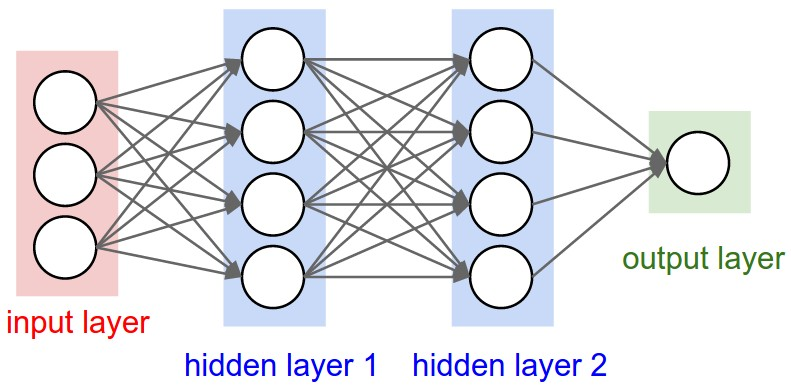
\includegraphics[width=0.6\linewidth]{figslides/nn.jpeg}}
  \caption{
  A regular 3-layer Neural Network.
  }
\end{figure}
%\clearpage % flush figures 


% !split
\subsection*{3D volumes of neurons}

Convolutional Neural Networks take advantage of the fact that the
input consists of images and they constrain the architecture in a more
sensible way. 

In particular, unlike a regular Neural Network, the
layers of a CNN have neurons arranged in 3 dimensions: width,
height, depth. (Note that the word depth here refers to the third
dimension of an activation volume, not to the depth of a full Neural
Network, which can refer to the total number of layers in a network.)

To understand it better, the above example of an image 
with an input volume of
activations has dimensions $32\times 32\times 3$ (width, height,
depth respectively). 

The neurons in a layer will
only be connected to a small region of the layer before it, instead of
all of the neurons in a fully-connected manner. Moreover, the final
output layer could  for this specific image have dimensions $1\times 1 times 10$, 
because by the
end of the CNN architecture we will reduce the full image into a
single vector of class scores, arranged along the depth
dimension. 


\begin{figure}[!ht]  % 
  \centerline{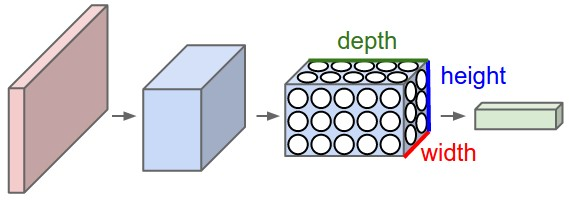
\includegraphics[width=0.6\linewidth]{figslides/cnn.jpeg}}
  \caption{
  A CNN arranges its neurons in three dimensions (width, height, depth), as visualized in one of the layers. Every layer of a CNN transforms the 3D input volume to a 3D output volume of neuron activations. In this example, the red input layer holds the image, so its width and height would be the dimensions of the image, and the depth would be 3 (Red, Green, Blue channels).
  }
\end{figure}
%\clearpage % flush figures 




% !split 
\subsection*{Layers used to build CNNs}


A simple CNN is a sequence of layers, and every layer of a CNN
transforms one volume of activations to another through a
differentiable function. We use three main types of layers to build
CNN architectures: Convolutional Layer, Pooling Layer, and
Fully-Connected Layer (exactly as seen in regular Neural Networks). We
will stack these layers to form a full CNN architecture.

A simple CNN for image classification could have the architecture:

\begin{itemize}
\item \textbf{INPUT} ($32\times 32 \times 3$) will hold the raw pixel values of the image, in this case an image of width 32, height 32, and with three color channels R,G,B.

\item \textbf{CONV} (convolutional )layer will compute the output of neurons that are connected to local regions in the input, each computing a dot product between their weights and a small region they are connected to in the input volume. This may result in volume such as $[32\times 32\times 12]$ if we decided to use 12 filters.

\item \textbf{RELU} layer will apply an elementwise activation function, such as the $max(0,x)$ thresholding at zero. This leaves the size of the volume unchanged ($[32\times 32\times 12]$).

\item \textbf{POOL} (pooling) layer will perform a downsampling operation along the spatial dimensions (width, height), resulting in volume such as $[16\times 16\times 12]$.

\item \textbf{FC} (i.e.~fully-connected) layer will compute the class scores, resulting in volume of size $[1\times 1\times 10]$, where each of the 10 numbers correspond to a class score, such as among the 10 categories of the MNIST images we considered above . As with ordinary Neural Networks and as the name implies, each neuron in this layer will be connected to all the numbers in the previous volume.
\end{itemize}

\noindent
% !split
\subsection*{Transforming images}

CNNs transform the original image layer by layer from the original
pixel values to the final class scores. 

Observe that some layers contain
parameters and other don’t. In particular, the CNN layers perform
transformations that are a function of not only the activations in the
input volume, but also of the parameters (the weights and biases of
the neurons). On the other hand, the RELU/POOL layers will implement a
fixed function. The parameters in the CONV/FC layers will be trained
with gradient descent so that the class scores that the CNN computes
are consistent with the labels in the training set for each image.


% !split
\subsection*{CNNs in brief}

In summary:

\begin{itemize}
\item A CNN architecture is in the simplest case a list of Layers that transform the image volume into an output volume (e.g.~holding the class scores)

\item There are a few distinct types of Layers (e.g.~CONV/FC/RELU/POOL are by far the most popular)

\item Each Layer accepts an input 3D volume and transforms it to an output 3D volume through a differentiable function

\item Each Layer may or may not have parameters (e.g.~CONV/FC do, RELU/POOL don’t)

\item Each Layer may or may not have additional hyperparameters (e.g.~CONV/FC/POOL do, RELU doesn’t)
\end{itemize}

\noindent
For more material on convolutional networks, we strongly recommend
the course
\href{{https://www.uio.no/studier/emner/matnat/ifi/IN5400/index-eng.html}}{IN5400 – Machine Learning for Image Analysis}
and the slides of \href{{http://cs231n.github.io/convolutional-networks/}}{CS231} which is taught at Stanford University (consistently ranked as one of the top computer science programs in the world). \href{{http://neuralnetworksanddeeplearning.com/chap6.html}}{Michael Nielsen's book is a must read, in particular chapter 6 which deals with CNNs}.


% !split
\subsection*{CNNs in more detail, building convolutional neural networks in Tensorflow and Keras}


As discussed above, CNNs are neural networks built from the assumption that the inputs
to the network are 2D images. This is important because the number of features or pixels in images
grows very fast with the image size, and an enormous number of weights and biases are needed in order to build an accurate network.  

As before, we still have our input, a hidden layer and an output. What's novel about convolutional networks
are the \textbf{convolutional} and \textbf{pooling} layers stacked in pairs between the input and the hidden layer.
In addition, the data is no longer represented as a 2D feature matrix, instead each input is a number of 2D
matrices, typically 1 for each color dimension (Red, Green, Blue). 


% !split
\subsection*{Setting it up}

It means that to represent the entire
dataset of images, we require a 4D matrix or \textbf{tensor}. This tensor has the dimensions:  
\[  
(n_{inputs},\, n_{pixels, width},\, n_{pixels, height},\, depth) .
\]

% !split
\subsection*{The MNIST dataset again}

The MNIST dataset consists of grayscale images with a pixel size of
$28\times 28$, meaning we require $28 \times 28 = 724$ weights to each
neuron in the first hidden layer.

If we were to analyze images of size $128\times 128$ we would require
$128 \times 128 = 16384$ weights to each neuron. Even worse if we were
dealing with color images, as most images are, we have an image matrix
of size $128\times 128$ for each color dimension (Red, Green, Blue),
meaning 3 times the number of weights $= 49152$ are required for every
single neuron in the first hidden layer.


% !split
\subsection*{Strong correlations}
Images typically have strong local correlations, meaning that a small
part of the image varies little from its neighboring regions. If for
example we have an image of a blue car, we can roughly assume that a
small blue part of the image is surrounded by other blue regions.

Therefore, instead of connecting every single pixel to a neuron in the
first hidden layer, as we have previously done with deep neural
networks, we can instead connect each neuron to a small part of the
image (in all 3 RGB depth dimensions).  The size of each small area is
fixed, and known as a \href{{https://en.wikipedia.org/wiki/Receptive_field}}{receptive}.


% !split 
\subsection*{Layers of a CNN}
The layers of a convolutional neural network arrange neurons in 3D: width, height and depth.  
The input image is typically a square matrix of depth 3. 

A \textbf{convolution} is performed on the image which outputs
a 3D volume of neurons. The weights to the input are arranged in a number of 2D matrices, known as \textbf{filters}.


Each filter slides along the input image, taking the dot product
between each small part of the image and the filter, in all depth
dimensions. This is then passed through a non-linear function,
typically the \textbf{Rectified Linear (ReLu)} function, which serves as the
activation of the neurons in the first convolutional layer. This is
further passed through a \textbf{pooling layer}, which reduces the size of the
convolutional layer, e.g.~by taking the maximum or average across some
small regions, and this serves as input to the next convolutional
layer.


% !split
\subsection*{Systematic reduction}

By systematically reducing the size of the input volume, through
convolution and pooling, the network should create representations of
small parts of the input, and then from them assemble representations
of larger areas.  The final pooling layer is flattened to serve as
input to a hidden layer, such that each neuron in the final pooling
layer is connected to every single neuron in the hidden layer. This
then serves as input to the output layer, e.g.~a softmax output for
classification.


% !split
\subsection*{Prerequisites: Collect and pre-process data}
\begin{minted}[fontsize=\fontsize{9pt}{9pt},linenos=false,mathescape,baselinestretch=1.0,fontfamily=tt,xleftmargin=7mm]{python}
# import necessary packages
import numpy as np
import matplotlib.pyplot as plt
from sklearn import datasets


# ensure the same random numbers appear every time
np.random.seed(0)

# display images in notebook
%matplotlib inline
plt.rcParams['figure.figsize'] = (12,12)


# download MNIST dataset
digits = datasets.load_digits()

# define inputs and labels
inputs = digits.images
labels = digits.target

# RGB images have a depth of 3
# our images are grayscale so they should have a depth of 1
inputs = inputs[:,:,:,np.newaxis]

print("inputs = (n_inputs, pixel_width, pixel_height, depth) = " + str(inputs.shape))
print("labels = (n_inputs) = " + str(labels.shape))


# choose some random images to display
n_inputs = len(inputs)
indices = np.arange(n_inputs)
random_indices = np.random.choice(indices, size=5)

for i, image in enumerate(digits.images[random_indices]):
    plt.subplot(1, 5, i+1)
    plt.axis('off')
    plt.imshow(image, cmap=plt.cm.gray_r, interpolation='nearest')
    plt.title("Label: %d" % digits.target[random_indices[i]])
plt.show()
\end{minted}


% !split
\subsection*{Importing Keras and Tensorflow}
\begin{minted}[fontsize=\fontsize{9pt}{9pt},linenos=false,mathescape,baselinestretch=1.0,fontfamily=tt,xleftmargin=7mm]{python}
from keras.utils import to_categorical
from sklearn.model_selection import train_test_split

# representation of labels
labels = to_categorical(labels)

# split into train and test data
# one-liner from scikit-learn library
train_size = 0.8
test_size = 1 - train_size
X_train, X_test, Y_train, Y_test = train_test_split(inputs, labels, train_size=train_size,
                                                    test_size=test_size)
\end{minted}

% !split
\subsection*{Using TensorFlow backend}

We need to define model and architecture and choose cost function and optmizer.
\begin{Verbatim}[numbers=none,fontsize=\fontsize{9pt}{9pt},baselinestretch=0.95]

import tensorflow as tf

class ConvolutionalNeuralNetworkTensorflow:
    def __init__(
        self,
        X_train,
        Y_train,
        X_test,
        Y_test,
        n_filters=10,
        n_neurons_connected=50,
        n_categories=10,
        receptive_field=3,
        stride=1,
        padding=1,
        epochs=10,
        batch_size=100,
        eta=0.1,
        lmbd=0.0,
    ):
        
        self.global_step = tf.Variable(0, dtype=tf.int32, trainable=False, name='global_step')
        
        self.X_train = X_train
        self.Y_train = Y_train
        self.X_test = X_test
        self.Y_test = Y_test
        
        self.n_inputs, self.input_width, self.input_height, self.depth = X_train.shape
        
        self.n_filters = n_filters
        self.n_downsampled = int(self.input_width*self.input_height*n_filters / 4)
        self.n_neurons_connected = n_neurons_connected
        self.n_categories = n_categories
        
        self.receptive_field = receptive_field
        self.stride = stride
        self.strides = [stride, stride, stride, stride]
        self.padding = padding
        
        self.epochs = epochs
        self.batch_size = batch_size
        self.iterations = self.n_inputs // self.batch_size
        self.eta = eta
        self.lmbd = lmbd
        
        self.create_placeholders()
        self.create_CNN()
        self.create_loss()
        self.create_optimiser()
        self.create_accuracy()
    
    def create_placeholders(self):
        with tf.name_scope('data'):
            self.X = tf.placeholder(tf.float32, shape=(None, self.input_width, self.input_height, self.depth), name='X_data')
            self.Y = tf.placeholder(tf.float32, shape=(None, self.n_categories), name='Y_data')
    
    def create_CNN(self):
        with tf.name_scope('CNN'):
            
            # Convolutional layer
            self.W_conv = self.weight_variable([self.receptive_field, self.receptive_field, self.depth, self.n_filters], name='conv', dtype=tf.float32)
            b_conv = self.weight_variable([self.n_filters], name='conv', dtype=tf.float32)
            z_conv = tf.nn.conv2d(self.X, self.W_conv, self.strides, padding='SAME', name='conv') + b_conv
            a_conv = tf.nn.relu(z_conv)
            
            # 2x2 max pooling
            a_pool = tf.nn.max_pool(a_conv, [1, 2, 2, 1], [1, 2, 2, 1], padding='SAME', name='pool')
            
            # Fully connected layer
            a_pool_flat = tf.reshape(a_pool, [-1, self.n_downsampled])
            self.W_fc = self.weight_variable([self.n_downsampled, self.n_neurons_connected], name='fc', dtype=tf.float32)
            b_fc = self.bias_variable([self.n_neurons_connected], name='fc', dtype=tf.float32)
            a_fc = tf.nn.relu(tf.matmul(a_pool_flat, self.W_fc) + b_fc)
            
            # Output layer
            self.W_out = self.weight_variable([self.n_neurons_connected, self.n_categories], name='out', dtype=tf.float32)
            b_out = self.bias_variable([self.n_categories], name='out', dtype=tf.float32)
            self.z_out = tf.matmul(a_fc, self.W_out) + b_out
    
    def create_loss(self):
        with tf.name_scope('loss'):
            softmax_loss = tf.reduce_mean(tf.nn.softmax_cross_entropy_with_logits_v2(labels=self.Y, logits=self.z_out))
            
            regularizer_loss_conv = tf.nn.l2_loss(self.W_conv)
            regularizer_loss_fc = tf.nn.l2_loss(self.W_fc)
            regularizer_loss_out = tf.nn.l2_loss(self.W_out)
            regularizer_loss = self.lmbd*(regularizer_loss_conv + regularizer_loss_fc + regularizer_loss_out)
            
            self.loss = softmax_loss + regularizer_loss

    def create_accuracy(self):
        with tf.name_scope('accuracy'):
            probabilities = tf.nn.softmax(self.z_out)
            predictions = tf.argmax(probabilities, 1)
            labels = tf.argmax(self.Y, 1)
            
            correct_predictions = tf.equal(predictions, labels)
            correct_predictions = tf.cast(correct_predictions, tf.float32)
            self.accuracy = tf.reduce_mean(correct_predictions)
    
    def create_optimiser(self):
        with tf.name_scope('optimizer'):
            self.optimizer = tf.train.GradientDescentOptimizer(learning_rate=self.eta).minimize(self.loss, global_step=self.global_step)
            
    def weight_variable(self, shape, name='', dtype=tf.float32):
        initial = tf.truncated_normal(shape, stddev=0.1)
        return tf.Variable(initial, name=name, dtype=dtype)
    
    def bias_variable(self, shape, name='', dtype=tf.float32):
        initial = tf.constant(0.1, shape=shape)
        return tf.Variable(initial, name=name, dtype=dtype)

    def fit(self):
        data_indices = np.arange(self.n_inputs)

        with tf.Session() as sess:
            sess.run(tf.global_variables_initializer())
            for i in range(self.epochs):
                for j in range(self.iterations):
                    chosen_datapoints = np.random.choice(data_indices, size=self.batch_size, replace=False)
                    batch_X, batch_Y = self.X_train[chosen_datapoints], self.Y_train[chosen_datapoints]
            
                    sess.run([CNN.loss, CNN.optimizer],
                        feed_dict={CNN.X: batch_X,
                                   CNN.Y: batch_Y})
                    accuracy = sess.run(CNN.accuracy,
                        feed_dict={CNN.X: batch_X,
                                   CNN.Y: batch_Y})
                    step = sess.run(CNN.global_step)
    
            self.train_loss, self.train_accuracy = sess.run([CNN.loss, CNN.accuracy],
                feed_dict={CNN.X: self.X_train,
                           CNN.Y: self.Y_train})
        
            self.test_loss, self.test_accuracy = sess.run([CNN.loss, CNN.accuracy],
                feed_dict={CNN.X: self.X_test,
                           CNN.Y: self.Y_test})
\end{Verbatim}

% !split
\subsection*{Train the model}

We need now to train the model, evaluate it and test its performance on test data, and eventually include hyperparameters.
\begin{minted}[fontsize=\fontsize{9pt}{9pt},linenos=false,mathescape,baselinestretch=1.0,fontfamily=tt,xleftmargin=7mm]{python}
epochs = 100
batch_size = 100
n_filters = 10
n_neurons_connected = 50
n_categories = 10

eta_vals = np.logspace(-5, 1, 7)
lmbd_vals = np.logspace(-5, 1, 7)
CNN_tf = np.zeros((len(eta_vals), len(lmbd_vals)), dtype=object)
        
for i, eta in enumerate(eta_vals):
    for j, lmbd in enumerate(lmbd_vals):
        CNN = ConvolutionalNeuralNetworkTensorflow(X_train, Y_train, X_test, Y_test,
                                      n_filters=n_filters, n_neurons_connected=n_neurons_connected,
                                      n_categories=n_categories, epochs=epochs, batch_size=batch_size,
                                      eta=eta, lmbd=lmbd)
        CNN.fit()
        
        print("Learning rate = ", eta)
        print("Lambda = ", lmbd)
        print("Test accuracy: %.3f" % CNN.test_accuracy)
        print()
            
        CNN_tf[i][j] = CNN
\end{minted}

% !split
\subsection*{Visualizing the results}

\begin{minted}[fontsize=\fontsize{9pt}{9pt},linenos=false,mathescape,baselinestretch=1.0,fontfamily=tt,xleftmargin=7mm]{python}
# visual representation of grid search
# uses seaborn heatmap, could probably do this in matplotlib
import seaborn as sns

sns.set()

train_accuracy = np.zeros((len(eta_vals), len(lmbd_vals)))
test_accuracy = np.zeros((len(eta_vals), len(lmbd_vals)))

for i in range(len(eta_vals)):
    for j in range(len(lmbd_vals)):
        CNN = CNN_tf[i][j]

        train_accuracy[i][j] = CNN.train_accuracy
        test_accuracy[i][j] = CNN.test_accuracy

        
fig, ax = plt.subplots(figsize = (10, 10))
sns.heatmap(train_accuracy, annot=True, ax=ax, cmap="viridis")
ax.set_title("Training Accuracy")
ax.set_ylabel("$\eta$")
ax.set_xlabel("$\lambda$")
plt.show()

fig, ax = plt.subplots(figsize = (10, 10))
sns.heatmap(test_accuracy, annot=True, ax=ax, cmap="viridis")
ax.set_title("Test Accuracy")
ax.set_ylabel("$\eta$")
ax.set_xlabel("$\lambda$")
plt.show()
\end{minted}

% !split 
\subsection*{Running with Keras}

\begin{minted}[fontsize=\fontsize{9pt}{9pt},linenos=false,mathescape,baselinestretch=1.0,fontfamily=tt,xleftmargin=7mm]{python}
from keras.models import Sequential
from keras.layers.convolutional import Conv2D
from keras.layers.convolutional import MaxPooling2D
from keras.layers import Flatten
from keras.layers import Dense
from keras.regularizers import l2
from keras.optimizers import SGD

def create_convolutional_neural_network_keras(input_shape, receptive_field,
                                              n_filters, n_neurons_connected, n_categories,
                                              eta, lmbd):
    model = Sequential()
    model.add(Conv2D(n_filters, (receptive_field, receptive_field), input_shape=input_shape, padding='same',
              activation='relu', kernel_regularizer=l2(lmbd)))
    model.add(MaxPooling2D(pool_size=(2, 2)))
    model.add(Flatten())
    model.add(Dense(n_neurons_connected, activation='relu', kernel_regularizer=l2(lmbd)))
    model.add(Dense(n_categories, activation='softmax', kernel_regularizer=l2(lmbd)))
    
    sgd = SGD(lr=eta)
    model.compile(loss='categorical_crossentropy', optimizer=sgd, metrics=['accuracy'])
    
    return model

epochs = 100
batch_size = 100
input_shape = X_train.shape[1:4]
receptive_field = 3
n_filters = 10
n_neurons_connected = 50
n_categories = 10

eta_vals = np.logspace(-5, 1, 7)
lmbd_vals = np.logspace(-5, 1, 7)
\end{minted}

% !split
\subsection*{Final part}

\begin{minted}[fontsize=\fontsize{9pt}{9pt},linenos=false,mathescape,baselinestretch=1.0,fontfamily=tt,xleftmargin=7mm]{python}
CNN_keras = np.zeros((len(eta_vals), len(lmbd_vals)), dtype=object)
        
for i, eta in enumerate(eta_vals):
    for j, lmbd in enumerate(lmbd_vals):
        CNN = create_convolutional_neural_network_keras(input_shape, receptive_field,
                                              n_filters, n_neurons_connected, n_categories,
                                              eta, lmbd)
        CNN.fit(X_train, Y_train, epochs=epochs, batch_size=batch_size, verbose=0)
        scores = CNN.evaluate(X_test, Y_test)
        
        CNN_keras[i][j] = CNN
        
        print("Learning rate = ", eta)
        print("Lambda = ", lmbd)
        print("Test accuracy: %.3f" % scores[1])
        print()
\end{minted}

% !split
\subsection*{Final visualization}

\begin{Verbatim}[numbers=none,fontsize=\fontsize{9pt}{9pt},baselinestretch=0.95]
# visual representation of grid search
# uses seaborn heatmap, could probably do this in matplotlib
import seaborn as sns

sns.set()

train_accuracy = np.zeros((len(eta_vals), len(lmbd_vals)))
test_accuracy = np.zeros((len(eta_vals), len(lmbd_vals)))

for i in range(len(eta_vals)):
    for j in range(len(lmbd_vals)):
        CNN = CNN_keras[i][j]

        train_accuracy[i][j] = CNN.evaluate(X_train, Y_train)[1]
        test_accuracy[i][j] = CNN.evaluate(X_test, Y_test)[1]

        
fig, ax = plt.subplots(figsize = (10, 10))
sns.heatmap(train_accuracy, annot=True, ax=ax, cmap="viridis")
ax.set_title("Training Accuracy")
ax.set_ylabel("$\eta$")
ax.set_xlabel("$\lambda$")
plt.show()

fig, ax = plt.subplots(figsize = (10, 10))
sns.heatmap(test_accuracy, annot=True, ax=ax, cmap="viridis")
ax.set_title("Test Accuracy")
ax.set_ylabel("$\eta$")
ax.set_xlabel("$\lambda$")
plt.show()
\end{Verbatim}

% !split
\subsection*{Fun links}

\begin{enumerate}
\item \href{{https://arxiv.org/abs/1604.07316}}{Self-Driving cars using a convolutional neural network}

\item \href{{https://deepdreamgenerator.com/}}{Abstract art using convolutional neural networks}
\end{enumerate}

\noindent

% ------------------- end of main content ---------------

\end{document}

